% This must be in the first 5 lines to tell arXiv to use pdfLaTeX, which is strongly recommended.
\pdfoutput=1
% In particular, the hyperref package requires pdfLaTeX in order to break URLs across lines.

\documentclass[11pt]{article}

% Change "review" to "final" to generate the final (sometimes called camera-ready) version.
% Change to "preprint" to generate a non-anonymous version with page numbers.
% \usepackage[review]{acl}
\usepackage[preprint]{acl}

% Standard package includes
\usepackage{times}
\usepackage{latexsym}

% For proper rendering and hyphenation of words containing Latin characters (including in bib files)
\usepackage[T1]{fontenc}
% For Vietnamese characters
% \usepackage[T5]{fontenc}
% See https://www.latex-project.org/help/documentation/encguide.pdf for other character sets

% This assumes your files are encoded as UTF8
\usepackage[utf8]{inputenc}

% This is not strictly necessary, and may be commented out,
% but it will improve the layout of the manuscript,
% and will typically save some space.
\usepackage{microtype}

% This is also not strictly necessary, and may be commented out.
% However, it will improve the aesthetics of text in
% the typewriter font.
\usepackage{inconsolata}

%Including images in your LaTeX document requires adding
%additional package(s)
\usepackage{graphicx}

% If the title and author information does not fit in the area allocated, uncomment the following
%
%\setlength\titlebox{<dim>}
%
% and set <dim> to something 5cm or larger.

\usepackage{color, xcolor}
\usepackage{booktabs}
\usepackage{multicol}
\usepackage{multirow, makecell, caption}
\usepackage{colortbl}
\usepackage{tikz}
\usepackage{arydshln}
\usepackage{pgfplots}
\usepackage{amsmath}
\usepackage{amssymb}

\usepackage{tabularx}
\usepackage{enumerate}

\makeatletter
\def\adl@drawiv#1#2#3{%
        \hskip.5\tabcolsep
        \xleaders#3{#2.5\@tempdimb #1{1}#2.5\@tempdimb}%
                #2\z@ plus1fil minus1fil\relax
        \hskip.5\tabcolsep}
\newcommand{\cdashlinelr}[1]{%
  \noalign{\vskip\aboverulesep
           \global\let\@dashdrawstore\adl@draw
           \global\let\adl@draw\adl@drawiv}
  \cdashline{#1}
  \noalign{\global\let\adl@draw\@dashdrawstore
           \vskip\belowrulesep}}
\makeatother

\title{Order Matters: Investigate the Position Bias in Multi-constraint Instruction Following}

% Author information can be set in various styles:
% For several authors from the same institution:
% \author{Author 1 \and ... \and Author n \\
%         Address line \\ ... \\ Address line}
% if the names do not fit well on one line use
%         Author 1 \\ {\bf Author 2} \\ ... \\ {\bf Author n} \\
% For authors from different institutions:
% \author{Author 1 \\ Address line \\  ... \\ Address line
%         \And  ... \And
%         Author n \\ Address line \\ ... \\ Address line}
% To start a separate ``row'' of authors use \AND, as in
% \author{Author 1 \\ Address line \\  ... \\ Address line
%         \AND
%         Author 2 \\ Address line \\ ... \\ Address line \And
%         Author 3 \\ Address line \\ ... \\ Address line}

\author{
    Jie Zeng\textsuperscript{1}, Qianyu He\textsuperscript{1}, Qingyu Ren\textsuperscript{1,3}, Jiaqing Liang\textsuperscript{2\textdagger}, Yanghua Xiao\textsuperscript{1\textdagger}\\\textbf{Weikang Zhou\textsuperscript{3}, Zeye Sun\textsuperscript{3}, Fei Yu\textsuperscript{3}}\\
    \\
    \textsuperscript{1}Shanghai Key Laboratory of Data Science, School of Computer Science, Fudan University \\
    \textsuperscript{2}School of Data Science, Fudan University  \textsuperscript{3}Ant Group\\
    \{jzeng23, qyhe21, qyren24\}@m.fudan.edu.cn, \{liangjiaqing, shawyh\}@fudan.edu.cn\\
}

%\author{
%  \textbf{First Author\textsuperscript{1}},
%  \textbf{Second Author\textsuperscript{1,2}},
%  \textbf{Third T. Author\textsuperscript{1}},
%  \textbf{Fourth Author\textsuperscript{1}},
%\\
%  \textbf{Fifth Author\textsuperscript{1,2}},
%  \textbf{Sixth Author\textsuperscript{1}},
%  \textbf{Seventh Author\textsuperscript{1}},
%  \textbf{Eighth Author \textsuperscript{1,2,3,4}},
%\\
%  \textbf{Ninth Author\textsuperscript{1}},
%  \textbf{Tenth Author\textsuperscript{1}},
%  \textbf{Eleventh E. Author\textsuperscript{1,2,3,4,5}},
%  \textbf{Twelfth Author\textsuperscript{1}},
%\\
%  \textbf{Thirteenth Author\textsuperscript{3}},
%  \textbf{Fourteenth F. Author\textsuperscript{2,4}},
%  \textbf{Fifteenth Author\textsuperscript{1}},
%  \textbf{Sixteenth Author\textsuperscript{1}},
%\\
%  \textbf{Seventeenth S. Author\textsuperscript{4,5}},
%  \textbf{Eighteenth Author\textsuperscript{3,4}},
%  \textbf{Nineteenth N. Author\textsuperscript{2,5}},
%  \textbf{Twentieth Author\textsuperscript{1}}
%\\
%\\
%  \textsuperscript{1}Affiliation 1,
%  \textsuperscript{2}Affiliation 2,
%  \textsuperscript{3}Affiliation 3,
%  \textsuperscript{4}Affiliation 4,
%  \textsuperscript{5}Affiliation 5
%\\
%  \small{
%    \textbf{Correspondence:} \href{mailto:email@domain}{email@domain}
%  }
%}

\begin{document}
\maketitle

\begin{abstract}

\begin{abstract}
% We present a learning-based method for multiple human rendering from sparse sets of multi-view images. Most current works are focused on single human settings that deliver accurate geometry and appearance using implicit neural representations. However, extending these methods for estimating multiple humans from sparse images remains challenging due to additional occlusion and clutter of multiple humans and the limited number of input views. We propose a neural implicit reconstruction method that addresses the inherent challenges. First, we propose to use geometry constraints by exploiting pre-computed meshes using a human body model (SMPL). Specifically, we regularize the signed distances using the SMPL mesh and leverage bounding boxes for improved rendering. Second, we propose a patch-based ray regularization to minimize rendering inconsistencies and a saturation regularization for robust optimization in variable illumination. Extensive experiments on both real-world and synthetic datasets demonstrate the benefits of our approach and show state-of-the-art performance against existing neural reconstruction methods. 

We present a method for recovering the shape and radiance of a scene consisting of multiple people given solely a few images. 
Multi-human scenes are complex due to additional occlusion and clutter. For single-human settings, existing approaches using implicit neural representations have achieved impressive results that deliver accurate geometry and appearance. 
However, it remains challenging to extend these methods for estimating multiple humans from sparse views. 
We propose a neural implicit reconstruction method that addresses the inherent challenges of this task through the following contributions: First, we propose to use geometry constraints by exploiting pre-computed meshes using a human body model (SMPL). Specifically, we regularize the signed distances using the SMPL mesh and leverage bounding boxes for improved rendering. Second, we propose a ray regularization scheme to minimize rendering inconsistencies, and a saturation regularization for robust optimization in variable illumination.  Extensive experiments on both real and synthetic datasets demonstrate the benefits of our approach and show state-of-the-art performance against existing neural reconstruction methods. 

% Finally, we demonstrate how our framework can be used for editing applications. 
\end{abstract}

% We present a neural learning method for multiple human reconstruction from a sparse set of camera views. Recent neural surface reconstruction methods could generate both 3D geometry and appearance, while usually fail to reconstruct consistent surfaces due to lacking of explicit multi-view geometry constraints, especially for complex scene(\eg multiple human). {\bf Previous works demonstrated that using geometry priors for simple objects significantly enhance the quality of the surfaces. In this work, we propose to extend this idea to using human body model (\eg SMPL) priors, represented by signed distance functions (SDF).} However, since human SMPL usually lacks sufficient details (\eg hair, cloth), we estimate SDF together with its' uncertainty for explicit smooth geometry regularization. In addition, we propose a patch based ray regularization to minimizes potential reconstruction inconsistency and saturation regularization for robust optimization in variable illuminations.  Our evaluations on both real human dataset (CMU Panoptic Dataset\cite{Simon_2017_CVPR,Joo_2017_TPAMI}) and synthetic data (THUman2.0 Dataset and MultiHuman-Dataset \cite{tao2021function4d,zheng2021deepmulticap} demonstrate state-of-the-art performance quantitatively and qualitatively. Extensive experiments show our methods enable a variety editing applications in 3D space without additional assistance of depth, masks, or segmentation.

%Existing multi-person reconstruction is often based on human models, which could reconstruct complex geometry but lose rendering quality due to lacking hair and clothing detail. Recently, volumetric rendering (\eg NeRF\cite{mildenhall2020nerf}) demonstrate promising rendering quality on novel views synthesis from dense input views, while reconstructing fidelity surfaces remains a challenge. Moreover, surface presentation methods \cite{yariv2021volume,wang2021neus} explore surface reconstruction during volume rendering, but it's still hard to handle occlusions and complex geometry (\eg multi-human) from sparse input views. Our methods take the advantages of the human model(\eg SMPL), recent volumetric rendering and scene representation methods. Specifically,we define our multi-human SMPL's surfaces as a zero-level set of a signed distance function (SDF) and train a neural SDF representation. We show how to incorporate this representation in point sampling, neural rendering and reconstruction, and propose a joint optimization for non-rigid shapes (\egclothed humans). Finally,

% We present a learning-based method for reconstructing multiple humans from a sparse set of camera views. Current surface reconstruction methods can generate geometry and appearance simultaneously, but suffer to reconstruct 3D consistent surfaces due to a lack of explicit multi-view geometric constraints, especially for complex scenes (e.g. multiple humans). Previous works show that the use of geometric priors for simple objects (or single scenes) significantly improves the fidelity of reconstructed surfaces. Leveraging that, we propose the use of utilizing human body model (e.g. SMPL) priors, represented by signed distance functions (SDF). However, human SMPL often lacks sufficient details (e.g. hair, cloth), and thus, we estimate the SDF along with its uncertainty to obtain smooth geometry regularization. In addition, we propose a patch-based method for ray regularization to potentially minimize inconsistencies in the reconstruction and to enable saturation regularization to increase the robustness during the optimization of variable illuminations. Our evaluations on both real human datasets (CMU Panoptic Dataset [32, 63]) and synthetic data (THUman2.0 Dataset and MultiHuman Dataset [83, 94] demonstrate state-of-the-art performance quantitatively and qualitatively. Extensive experiments show that our method enables a variety of editing applications in 3D space without additional assistance of depth, masks, or segmentation.



\end{abstract}

\section{Introduction}\label{sec:intro}

\section{Introduction}
\label{sec:intro}

Human reconstruction from single images \cite{choutas2020monocular, kanazawa2018end,liu2022recent}, multiple images \cite{guo2019relightables, collet2015high}, RGB videos \cite{alldieck2018detailed,Kocabas20} or RGB-D data \cite{yu2017bodyfusion,yu2018doublefusion} has received a lot of attention, much less explored is the task of \emph{multiple} human scenario, which is essential for scene understanding, behavior modeling, collaborative augmented reality, and sports analysis.  
%
The multi-human setting introduces additional challenges, as there is now a higher level of occlusion and clutter 
which hinders matching and reconstruction. 
Although in principle one could approach this by first detecting and then independently processing each person, 
simultaneous reconstruction of multiple humans can help to globally reason about occlusion at the level of the scene~\cite{jiang2020coherent, sun2022putting}, 
%which has been shown to produce better results~\cite{jiang2020coherent, sun2022putting}, 
and can potentially recover coherent 3D spatial relations among the people.

Several recent works have attempted to recover multiple humans from a single view \cite{choi2022learning, sun2022putting, sun2021monocular, zanfir2018deep, zanfir2018monocular, fieraru2020three, jiang2020coherent, zhang2021body, ugrinovic2021body,mustafa2021multi}. However, the majority of these are based on regressing the parameters of a human body model --typically SMPL \cite{loper2015smpl}--
which provides coarse reconstructions that %cannot handle 
lack hair, clothing, and geometric details. 
Multi-view settings can help resolve some of the occlusions as well as depth ambiguities, but require a dense array of RGB cameras to achieve a detailed reconstruction \cite{collet2015high, joo2015panoptic,vlasic2009dynamic}.
% which is not easily accessible. % available. 
A more convenient capture system %that could in principle still deliver optimal results 
is the \emph{sparse} multi-view setting, where only a handful of cameras is required.
%, where the number of cameras is limited to 2-15. 
However, due to the decreased number of views and increased level of occlusion, 
existing methods require segmentation masks and a pre-scanned template mesh \cite{liu2011markerless, wu2013set}, rely on a coarse body model \cite{zhang2021lightweight, huang2021dynamic}, or require temporal information \cite{zheng2021deepmulticap, huang2021dynamic}.

A parallel line of work simultaneously tackles the novel-view-synthesis and geometry-reconstruction problems by combining neural coordinate-based representations, \eg implicit signed distance functions (SDFs) \cite{park2019deepsdf}, with differentiable rendering \cite{yariv2021volume,wang2021neus,yariv2020multiview,mildenhall2020nerf}. 
This approach has the advantage of producing, along with geometry, renderings from novel viewpoints that can capture complex surface/light interactions, increasing the scope of applications. 
NeRF~\cite{mildenhall2020nerf}, for example, uses volumetric rendering to produce impressive images under novel views, albeit at the cost of sub-optimal geometries due to the unconstrained volumetric representation. 
SDF-based methods \cite{yariv2021volume,wang2021neus,yariv2020multiview}, while delivering images of slightly lower quality, have been shown to produce 3D surfaces that are competitive with classical approaches. 
For humans, this has been leveraged to obtain geometry and appearance from monocular video \cite{jiang2022selfrecon,chen2021animatable}, RGB-D video \cite{dong2022pina}, and sparse multi-view video \cite{wang2022arah, liu2021neural, peng2021neural, zheng2021deepmulticap, kwon2021neural, peng2021animatable, xu2021h, weng2022humannerf}. 
%% NOTE: \cite{xu2021h} also has experiments for static sparse MV image
However, none of these works, with the exception of \cite{zheng2021deepmulticap,zhang2021editable}, were designed to handle the increased geometric complexity and occlusion of the multi-human case. 
%%%%%%%%%%%%%%%%%%%%%%%%%%%%%%%%%%%%%%%%%%%%%not the only work, STnerf, SIgsia2022 and deep multicap
Current works \cite{zheng2021deepmulticap,zhang2021editable} address the multi-human setting, but both require a set of videos, which effectively becomes a dense array of views as long as deformations are modeled correctly.
%DeepMultiCap \cite{zheng2021deepmulticap} is the only work that addresss the multi-human setting, but the method requires segmentation and was focused on reconstruction from videos, which effectively becomes a dense array of views as long as deformations are modeled correctly.

In this paper, we address the problem of multiple 3D human surfaces and volume rendering from sparse static multi-view images. Our key insight is that human-specific geometric constraints can be leveraged to tackle the challenging sparse-view setting.

Specifically, we first obtain a SMPL body model from the input data and use it to initialize the implicit SDF network, where we define the surface of a multi-human scene as the zero-level set of the SDF. 
Then, the geometry network is optimized with multi-view images by leveraging surface and volume rendering ~\cite{wang2021neus} along with uncertainty estimation methods \cite{deng2022depth,roessle2022dense}, where the SMPL meshes are treated as noisy estimations.  
% [to keep the method general for novel scenes, we do not rely on features pre-trained on a large dataset]
To achieve higher rendering quality from sparse training views, we additionally propose a patch-based regularization loss that guarantees consistency across different rays and a saturation regularization that ensures consistency for variable image illuminations within the same scene.% \va{I feel this is a problem that was not pointed out before, and it would be nice to elaborate better}.

We evaluate our method quantitatively and qualitatively on real multi-human (CMU Panoptic~\cite{Simon_2017_CVPR,Joo_2017_TPAMI}) and synthetic (MultiHuman~\cite{zheng2021deepmulticap}) datasets. We demonstrate results on 5,10,15 and 20 training views, where we achieve state-of-the-art performance in terms of surface reconstruction and novel view quality. 

%In summary, our contributions are: 
%\begin{itemize}
%\item We propose the first neural implicit surface and volume rendering for multiple humans from sparse static images; 
%\item We propose a novel geometric initialization and regularization based on human SMPL, which allows for multi-human rendering simultaneously; %To address the problem of occlusion, we propose the use of SMPL for geometric regularization; 
%\item We propose a patch-based ray consistency regularization and an image saturation regularization that ensures illumination consistency across views;
%\item Our method achieves state-of-the-art performance and the code will be public online. 
%\end{itemize}

%%%%%%%%%%%%%%%%%%%%%%
%% MOTIVATION
% Motivations for multi-human from the multi-human, single-view domain:
%       - A lot of occlusions, if only a crop of the person is used then SOTA methods might fail (\cite{choi2022learning})
%       - Simultanesouly considering multiple person has been empirically shown to work better \cte{all the works on mult-human SMPL}
%       - The reconstructions can be made coherent in 3D space, i.e. with correct relative depth among the people. Plausible 3D spatial relations.
% The problem with SMPL based methods is that they cannot reconstruct clothes, hair, etc

% Applications in behavior analysis, automatic video analysis of sport events, or collaborative augmented reality applications
% human-computer interaction, human behavioral modeling, assisted therapy, monitoring sports performances, protection and security, special effects, modeling and indexing archival footage, or self-driving cars. (this is for monocular)

% We take one step beyond SMPL and use implicit representations for more accurate reconstructions

% "The straightforward solution consists in regarding different people as independent instances and estimating the body shapes and poses one by one using a single-person approach. This strategy, however, may result in inconsistent spatial arrangements and erroneous poses of the reconstructed people." (re-phrase)

% *** Why we cannot do cut one person then reconstruct it --> there should be experiments, else be careful with claims

%%%%%%%%%%%%%%%%%%%%%%
%% STORY
%   - Reconstructing geometry from a scene with multiple humans is hard because of occlusions
%   - Multiple views can help disambiguate, but it's stil hard.
%       => most are single human. For multi-human one can detect and reconstruct, but this can fail - and matching detections among views might not be straight-forward (?) Also, computational time scales (linearly) with the number of people
%       => there are a few multi-human, but ?
%       => people resort to SMPL to make the problem more tractable
%           *** classic matching methods: problem with multi-humans??
%   - SMPL doesn't have clothes or hair so geometry sucks
%   - We consider in particular the scenario where only a sparse number of cameras is available; dense rigs are not easily accessible. Dense => expensive and sophisticated hardware setup and low run-time efficiency (re-phrase)
%   - To address this, we present a method for multi-human 3D reconstruction from multiple views based on neural rendering. 
%   - To handle the occlussions and sparse views, we first fit a SMPL model. Following the recent line of works that make use of geometric quantities to improve reconstruction, we propose to to initialize the reconstruction by building an SDF from the acquired SMPL models.
%   - 

%%%%%%%%%%%%%%%%%%%%%%
% Multi-view capture with dense views and/or temporal data demands a significant cost in time and money, with increased complexity of device requirements, synchronisation, data storage and transfer times. Consequently, 3D reconstruction from a sparse set of images has become an increasingly popular problem~\cite{niemeyer2022regnerf, kim2022infonerf,long2022sparseneus,dong2021shape}, more so after the recent progress in deep neural rendering and reconstruction approaches~\cite{mildenhall2020nerf, park2019deepsdf}. % However, it remains a difficult problem due to the sparsity of 3D cues, requiring carefully designed regularization losses~\cite{kim2022infonerf,niemeyer2022regnerf} or knowledge transfer from pre-trained networks~\cite{yu2021pixelnerf}. This cue scarcity problem becomes even worse when reconstructing cluttered scenes, such as those containing a multitude of people., due to increased occlusions.
% % Multi-view capture with dense views and/or temporal data entails significant capture device requirements, synchronisation, data storage and transfer challenges. Hence, being able to capture scenes from a mere set of static sparse images has become a more than ever popular problem \cite{niemeyer2022regnerf, kim2022infonerf,long2022sparseneus,dong2021shape} especially in the wake of deep learning. 
% Yet, the scarcity of 3D cues in such setups requires carefully designed regularization or knowledge transfer. This scarcity is exacerbated further with cluttered scenes, such as scenes containing a multitude of people.   

% 3D reconstruction of humans from single images \cite{choutas2020monocular, kanazawa2018end,liu2022recent}, multiple images \cite{guo2019relightables, collet2015high}, RGB videos \cite{alldieck2018detailed,Kocabas20} or RGB-D data \cite{yu2017bodyfusion,yu2018doublefusion} has received a lot of attention, much less explored is the task of \emph{multiple} human reconstruction, which is essential for scene understanding, behavior modeling, collaborative augmented reality, and sports analysis.  
% %
% The multi-human setting introduces additional challenges, as there is now a higher level of occlusion and clutter 
% which hinders matching and reconstruction. 
% Although in principle one could approach this by first detecting and then independently processing each person, 
% simultaneous reconstruction of multiple humans can help to globally reason about occlusion at the level of the scene~\cite{jiang2020coherent, sun2022putting}, 
% %which has been shown to produce better results~\cite{jiang2020coherent, sun2022putting}, 
% and can potentially recover coherent 3D spatial relations among the people. %, taking a step towards better scene understanding.
% % simultaneous reconstruction of multiple humans has several advantages. 
% % First, this strategy  allows to further recover coherent 3D spatial relations among the people, taking a step towards better scene understanding.
% % Second, the presence of multiple people can imply a high level of occlusion. While some works explicitly handle this case for single humans \cite{khirodkar2022occluded, zhang2020object}, globally reasoning about occlusion at the level of the scene has been shown to produce better results \cite{jiang2020coherent, sun2022putting}.  
% % Finally, the detect-and-reconstruct approach increases (linearly) in computational time with each new person. 

% % While 
% Several recent works have attempted to recover multiple humans from a single view \cite{choi2022learning, sun2022putting, sun2021monocular, zanfir2018deep, zanfir2018monocular, fieraru2020three, jiang2020coherent, zhang2021body, ugrinovic2021body,mustafa2021multi}. However, the majority of these are based on regressing the parameters of a human body model --typically SMPL \cite{loper2015smpl}--
% which provides coarse reconstructions that %cannot handle 
% lack hair, clothing, and geometric details. 
% Multi-view settings can help resolve some of the occlusions as well as depth ambiguities, but require a dense array of RGB cameras to achieve a detailed reconstruction \cite{collet2015high, joo2015panoptic,vlasic2009dynamic} 
% % which is not easily accessible. % available. 
% A more convenient capture system %that could in principle still deliver optimal results 
% is the \emph{sparse} multi-view setting, where only a handful of cameras is required.
% %, where the number of cameras is limited to 2-15. 
% However, due to the decreased number of views and increased level of occlusion, 
% existing methods require segmentation masks and a pre-scanned template mesh \cite{liu2011markerless, wu2013set}, rely on a coarse body model \cite{zhang2021lightweight, huang2021dynamic}, or require temporal information \cite{zheng2021deepmulticap, huang2021dynamic}.

% %%%\todo{pifu should go somewhere here... pifu is single human though. Goes into the recent line of work: pre-train on a large dataset and then at test time use sparse views: \cite{zheng2021deepmulicap}}


% % --> send the message that MV with SMPL is kind of solved, but we need to take the next step. 
% %but as shown by several works \cite{...}, this is not sufficient to solve the problem. In fact, % in effect, in practice, at bottom
% % "The first sparse for multi-humans" -> \cite{zhang2021lightweight}, 

% % In parallel, there has been development in neural 3D geometry reconstruction by using SDFs \cite{..} or volume-rendered SDFs \cite{...}. These are great but require many views. For the sparse view case, infonerf, regnerf, dietnerf. They show improved results, but as demonstrated here these are not sufficient for the multi-human reconstruction problem.




% %%%%\todo{improving geometry to improve rendering?}

% % Inspired by the success of NeRF~\cite{mildenhall2020nerf}, 
% A parallel line of work simultaneously tackles the novel-view-synthesis and geometry-reconstruction problems by combining neural coordinate-based representations, \eg implicit signed distance functions (SDFs) \cite{park2019deepsdf}, with differentiable rendering \cite{yariv2021volume,wang2021neus,yariv2020multiview,mildenhall2020nerf}. 
% This approach has the advantage of producing, along with geometry, renderings from novel viewpoints that can capture complex surface/light interactions, increasing the scope of applications. 
% NeRF~\cite{mildenhall2020nerf}, for example, uses volumetric rendering to produce impressive images under novel views, albeit at the cost of sub-optimal geometries due to the unconstrained volumetric representation. 
% SDF-based methods \cite{yariv2021volume,wang2021neus,yariv2020multiview}, while delivering images of slightly lower quality, have been shown to produce 3D surfaces that are competitive with classical approaches. 
% For humans, this has been leveraged to obtain geometry and appearance from monocular video \cite{jiang2022selfrecon,chen2021animatable}, RGB-D video \cite{dong2022pina}, and sparse multi-view video \cite{wang2022arah, liu2021neural, peng2021neural, zheng2021deepmulticap, kwon2021neural, peng2021animatable, xu2021h, weng2022humannerf}. 
% %% NOTE: \cite{xu2021h} also has experiments for static sparse MV images (single human)
% %% Monocular video: also "SelfNeRF: Fast Training NeRF for Human from Monocular Self-rotating Video". But this isn't published yet
% %
% However, 
% none of these works, with the exception of \cite{zheng2021deepmulticap}, were designed to handle the increased geometric complexity and occlusion of the multi-human case. DeepMultiCap \cite{zheng2021deepmulticap} is the only %multi-view neural reconstruction 
% work that addresss the multi-human setting, but the method requires a set of videos, which effectively becomes a dense array of views as long as deformations are modeled correctly.

% In this paper we address, for the first time, 
% the problem of reconstructing multiple 3D humans from a \emph{static} and \emph{sparse} set of cameras using neural implicit surfaces. 
% Our key insight is that human-specific geometric constraints can be leveraged to tackle the challenging sparse-view setting.
% %by first fitting  a SMPL body model to the input, building on top of the works 
% % building on the set of works that can faithfully disambiguate pose and shape for multiple people, but only deliver coarse reconstructions, \eg~\cite{huang2017towards,zhang2021lightweight}. %\va{This is a bit risky, since the way we get smpl is a bit shady (in practice, from dense MV cameras)}. 
% Specifically, we first obtain a SMPL body model from the input data, and use this to train a geometry-only implicit SDF network, where we define the surface of a multi-human scene as the zero-level set of the SDF. 
% In a second step, the geometry network is fine-tuned using multi-view images by leveraging the recently-proposed NeuS~\cite{wang2021neus} along with uncertainty-based rendering \cite{deng2022depth,roessle2022dense}, where the SMPL meshes are treated as noisy estimations.  
% % [to keep the method general for novel scenes, we do not rely on features pre-trained on a large dataset]
% To achieve higher rendering quality from sparse training views, we additionally propose a patch-based regularization loss 
% that guarantees consistency across different rays, and a saturation regularization that ensure consistency for variable image illuminations within a same scene.% \va{I feel this is a problem that was not pointed out before, and it would be nice to elaborate better}.

% We evaluate our method quantitatively and qualitatively on real multi-human (CMU Panoptic~\cite{Simon_2017_CVPR,Joo_2017_TPAMI}) and synthetic (MultiHuman~\cite{zheng2021deepmulticap}) datasets. We demonstrate results on 5,10,15 and 20 training views, where we achieve state-of-the-art performance in terms of surface reconstruction and image quality. %Another advantage is that the proposed geometry initialization enables more efficient learning.

% In summary, our contributions are: 
% % 1. We demonstrate an approach to use multiple human bodies as geometric regularization. We propose to use SDF along with estimated uncertainty as explicit geometry constraints, allowing the  learning of details. \\
% (1) We propose the first neural 
% implicit geometry and appearance reconstruction method for multiple humans using a sparse set of static views; 
% (2) To address the problem of occlusion, we propose the use SMPL for geometric regularization; 
% (3) To handle sparse views under occlusion, we propose a patch-based ray consistency regularization, and an image saturation regularization that ensures illumination consistency across views.

%  Code and models will be made available.
% 3.  \todo{I will re-phrase this after finishing the method. This needs to come before in the introduction, if it stays} We combine box rendering with editing, which enables editing multi-humans in 3D space during inference without using masks and segmentation, while preserving the detail and quality of rendered novel multi-human views.   \\



%%%%%%%%%%%%%%%%%%%%%%
% --------------------------------


% Multiple human reconstruction has been a popular and significant topic in computer vision and computer graphics, which enables various applications, such as Virtual Reality (VR) and Augmented Reality (AR), films, teleconferences, and so on. Researches for human reconstruction mainly consist of model-based and model-free, both of them has achieved tremendous progress in recent years. 

% Traditional model-based approaches utilize parametric human bodies (\eg human SMPL \cite{loper2015smpl}) or truncated signed distance fields (TSDFs) for human geometry reconstruction \cite{loper2015smpl,bhatnagar2020combining,liu2021neural,yu2017bodyfusion,yu2018doublefusion,peng2021neural}. %Though human SMPL could provide solid geometry notes, 
% While relying on the human model(\eg SMPL skinning weights of a naked body) may risk losing hair and clothing details. Model-free methods learns from a set of multi-view images or videos with loosing detail constraints \cite{peng2021neural,dong2022pina,peng2021neural,dong2022pina, liu2021neural}, allowing more realistic reconstructed details. With the recent progress of implicit neural representations\cite{sitzmann2019deepvoxels,xu2022point,wiles2020synsin, mildenhall2020nerf,zhang2020NeRF++}, many model-free methods utilize NeRF to achieve photo-realistic rendering. However, NeRF\cite{mildenhall2020nerf} based methods do not sufficiently constrain the 3D geometry, making them hard to reconstruct high-fidelity surfaces or accurate geometry. Further, most existing researches focus on single person reconstruction from videos \cite{peng2021neural,dong2022pina} or images\cite{peng2021neural,dong2022pina, liu2021neural}. For multiple human reconstructions from a single frame, the task becomes even harder to recover geometry and appearance with sufficient details due to multiple human scenes usually containing more complex geometry and occlusions. In this paper, we address those challenges by taking advantage of recent neural implicit surface reconstruction methods\cite{yariv2021volume,wang2021neus,yariv2020multiview} and human bodies models(\eg SMPL\cite{loper2015smpl}), reconstructing multi-human 3D geometry and appearance simultaneously. 

% Recent neural implicit surface reconstruction methods\cite{yariv2021volume,wang2021neus,yariv2020multiview} propose to use a signed distance function (SDF) to present the surface and combine SDF-based density function with volumetric rendering. They could learn an implicit SDF representation and reconstruct geometry and appearance simultaneously. However, the optimization of those methods still depends on direct color field and lack explicit geometry constraints, making them hard to reconstruct consistent geometry and appearance for unseen regions(\eg sparse input view) and occlusion areas (\eg multiple human scene). To alleviate those limitations, we propose to use a multiple human bodies models(SMPL) as geometry initialization, as well as to provide explicit geometry constraints.

% %\cite{yariv2021volume} uses volume density function as Laplace’s cumulative distribution function (CDF) for geometry representation, 
% %Neus\cite{wang2021neus} and Volsdf\cite{yariv2021volume} are among scene representation methodsuse signed distance functions (SDF) for surface representation and introduce the SDF-induced density function to enable the volume rendering to

% %More recently, with the rapidly progress of implicit neural representations\cite{sitzmann2019deepvoxels,xu2022point,wiles2020synsin, mildenhall2020nerf,zhang2020NeRF++}, many researches combine differentiable neural rendering with human bodies model \cite{liu2021neural,peng2021neural,dong2022pina}. Among those,  \cite{liu2021neural} combines human SMPL with implicit learning, and uses it as a proxy to unwarp the surrounding 3D space into a canonical pose, \cite{peng2021neural} could render detailed novel views (\eg with hair,cloths) of the human body from a set sparse input video. Thanks to neural radiance fields (NeRF\cite{mildenhall2020nerf}), those approaches could achieve photo-realistic rendering. However, NeRF\cite{mildenhall2020nerf} does not sufficiently constrain the 3D geometry, making those methods hard to reconstruct high-fidelity surfaces or accurate geometry.

% %Recent scene representation methods combines surface representation with neural volume rendering \cite{yariv2021volume,wang2021neus,yariv2020multiview}. % In order to achieve high quality surface reconstruction while retaining rendering quality, 
% %Among those, \cite{oechsle2021unisurf} proposes a unified framework to reconstruct solid objects from 2D image inputs, 

% Specifically, inspired by Neus\cite{wang2021neus} and Volsdf \cite{yariv2021volume}, we define the surface of multiple human SMPL as a zero-level set of a signed distance function (SDF)  and use it to train a neural SDF presentation as a geometry prior. However, relying on SDF sampled from SMPL directly may risk losing hair and clothing details. Thus, we learn SDF together with uncertainty and combine them together for explicit geometry regularization, which enables the learning of multiple person's clothing and hair details. In addition,
% to achieve higher rendering quality from sparse training views, we propose a patch-based regularization to guarantee consistency across different rays and saturation regularization to ensure image illumination consistency. 
% %retaining multi-view consistency remains a challenge for NeuS-related methods, especially for complex thin structures and large smooth regions. To tackle this challenge, we propose a patch-based ray regularization for photo-metric consistency and saturation regularization for image illumination consistency. 

% %Assuming this SDF presentation storing the multi-human geometry information, we incorporate this by re-initializing the follow-up neural network with the learned weights, utilizing the SDF value for the weights of hierarchical sampling \cite{mildenhall2020nerf} and volume rendering. Inspired by \cite{ortiz2022isdf, dong2022pina}, instead of using the SDF value sampled from SMPL to supervise the neural network learning directly(which consumes lots of time and lacks details), we propose a point-based SDF regularization allowing for the learning of multi-human clothing and hair details. Moreover, we present an approach for human editing during rendering, without additional training or information(\eg depth, mask or segmentation).   \\
% We evaluate our method on both real multi-human datasets (CMU Panoptic Dataset\cite{Simon_2017_CVPR,Joo_2017_TPAMI}) and synthetic data (THUman2.0 Dataset
% and MultiHuman-Dataset \cite{tao2021function4d,zheng2021deepmulticap}) both qualitatively and quantitatively. Specifically,  we demonstrate testing results on 10,15,20 training views,respectively, and achieve state-of-the-art performance on both real datasets and synthetic datasets. %Another advantage is that the proposed geometry initialization enables more efficient learning. 
% In summary, our contributions include:\\
% 1. We demonstrate an approach to use multiple human bodies as geometric initialization. We propose to use SDF along with estimated uncertainty as explicit geometry constraints, allowing the  learning of details. \\
% 2. We propose a patch-based KL regularization to ensure consistency across different rays and image saturation regularization for illumination consistency. \\
% 3. We combine box rendering with editing, which enables editing multi-humans in 3D space during inference without using masks and segmentation, while preserving the detail and quality of rendered novel multi-human views.   \\


\section{Related Work}

\section{Related Work}
In this section, we introduce the emerging concept of \emph{regional explanations} that inspired our tool, and discuss prior work on interpreting feature interactions and visual analytics in xAI.

\subsection{Regional methods}
Set between local and global methods,
an emerging category of explanation methods are regional methods, which focus on specific subgroups of the data. \textsc{Repid}~\cite{herbinger2022Repid} analyzes the ICE curves of a feature by identifying subgroups with different behaviors based on the shapes of individual instances' curves. A decision tree divides these groups while maintaining interpretable labels for easier understanding.

While \textsc{Repid} requires selecting an initial feature for exploring interactions, \textsc{Gadget}~\cite{herbinger2023decomposing} offers a more general approach by recursively decomposing the entire feature space to identify simple subspaces with minimal interactions, allowing for straightforward models in explanations. Like \textsc{Repid}, \textsc{Gadget} uses decision trees to guide the decomposition process.

Unlike \textsc{Finch}, \textsc{Repid} and \textsc{Gadget} do not identify feature interactions relevant to a specific instance; instead, they search for feature interactions globally by identifying subgroups.

\subsection{Feature Interaction Interpretation}
Few approaches exist for interpreting or visualizing higher-order feature interactions involving more than two features. Tsang et al.~\cite{tsang2021interpretable} provide a comprehensive review of feature interactions, emphasizing the need for improved interactive visualizations, which \textsc{Finch} aims to address. Zhang et al.~\cite{zhang2023capturing} take a mathematical approach, assuming product separability of feature interactions. Their method identifies these interactions and determines the most likely mathematical formula to represent them. Unlike \textsc{Finch}, this approach focuses on global feature interactions and is limited to this specific type of interaction. Friedman~\cite{friedman2024function} visualizes model interactions by breaking them down into a tree structure, allowing for the visualization of up to three features through line or bar charts. This tree provides a global overview of the interactions within the model, whereas \textsc{Finch} focuses on local feature interactions and can visualize interactions of more than three features.


Other approaches group features together, interpreting them as a unified group, which is especially useful for highly correlated features. For instance, Jullum et al.~\cite{jullum2021efficient} proposed computing Shapley values for groups rather than individual features. Ferretini et al.~\cite{ferrettini2022coalitional} also use grouping but as a step to enhance the calculation of final individual feature values. Going further, Mijolla et al.~\cite{mijolla2020human} propose an approach based on latent representations that redefine features as combinations of the original ones, making them easier for humans to understand. An automatic approach to latent representations are dimension reduction techniques like PCA, as demonstrated by Seedorff and Brown~\cite{seedorff2021totalvis}.

\subsection{Visual Analytics for xAI}

Our work aligns with a series of visual analytics tools designed for xAI. \textsc{Prospector}, by Krause et al.~\cite{krause2016interacting}, combines local and global explanation methods with an instance-centric interface. It builds on classical methods like PDPs but lacks functionality for higher-order feature interactions.

\textsc{Vine}, developed by Britton~\cite{britton2019vine}, is specifically designed to visualize feature interactions. Unlike \textsc{Finch}, it follows a global approach, clustering ICE curves for each feature, similar to \textsc{Repid}, and embedding this clustering in an overview and detailed views.

A similar approach was presented by Molnar et al.~\cite{molnar2023model}, who aimed to improve misleading PDPs by finding subgroups in the data with low feature interactions. Like \textsc{Gadget}, they compute a decision tree but visualize the results of each node in a PDP plot of a feature.



Hohman et al.~\cite{hohman2019gamut} designed a visual analytics system that offers various explanations for machine learning experts, although it does not cover higher-order interactions. They note that participants frequently switched between global and local explanations, highlighting the importance of interactivity.

Inglis et al.~\cite{Inglis2022Visualizing} present techniques for exploring pairwise interactions using matrix layouts of PDPs and network visualizations. \textsc{Finch} focuses on the visualization of interactions of even higher orders.


Lundberg et al.~\cite{lundberg2018consistent} created a VA system that uses SHAP force plots to visualize how different features influence the prediction for one instance over time on a clinical example. 
Their system visualizes all features in an independent manner, whilst ours shows their interaction.

\section{Method}

\subsection{Background}
In this paper, we mainly focus on the multi-constraint instruction $I_c$. It can be formulated as a seed instruction incorporated with ${n}$ constraints:
\begin{equation}
\label{eq1}
    I_c = I_s \oplus C_1 \oplus ... \oplus C_n,
\end{equation}
where the seed instructions $I_s$ describe a task, e.g., write a story, while these constraints $\sum_{i=1}^n C_i$ limit the output from different aspects, e.g., format, length, content, etc. $\oplus$ stands for the concatenation operation. 
% \footnote{We provide more examples of multi-constraint instruction in Appx.~\ref{appx:con_samp}.} 
% seed + 1 2 3 4


\subsection{Probing Task} \label{method}
% 我们尝试从约束的难度角度出发 量化指令中的不同排布情况 to achieve this, two problems need to be soluted: how to quantify the 
% 我们参考约束的分类建模
\subsubsection{Task Formulation}
To investigate the impact of constraint order, we introduce a probing task. In this task, the LLM is given multi-constraint instructions with constraints arranged in various orders. The LLM's task is to generate a response that follows all constraints. We evaluate the LLM in two practical scenarios: single-round and multi-round inference. The LLM's responses are then evaluated to determine its performance across various constraints. The overall procedure is illustrated in Fig.~\ref{fig:method}. In the following sections, we will provide a detailed explanation.





\subsubsection{Multi-constraint Instruction Synthesis}\label{sec:ins_cons}
To ensure the generalizability of probing data, we construct the initial multi-constraint instructions which include a variety of tasks and diverse constraint combinations. The multi-constraint instruction synthesis can be further divided into two parts: seed sampling and constraint sampling. 

For the seed sampling, we sample data from three source datasets: (1) Natural Instructions V2~\cite{wang2022supernaturalinstructions}. It is an instruction collection covering more than 1600 NLP tasks. We filter those tasks that are too easy and could potentially conflict with complex constraints, e.g., object classification and sentiment tagging. Then, we randomly sample 52 instructions from the remaining tasks. (2) Self-Instruct~\cite{wang2023self}. We only sample 83 instances from their initial 175 seed instructions which are formulated by humans. (3) Open Assistant~\cite{kopf2024openassistant}. Following the strategy of Suri~\cite{li2023self}, we filter out the first turn of the conversation with the highest quality (marked as rank 0 in the dataset) and sample 65 instances from them. Overall, we obtain 200 seed instructions, where the number of instructions is denoted as $n_{seed}$.

As for the constraint sampling, we first categorize the constraints into 8 groups with 25 fine-grained types~\cite{zhou2023instructionfollowing}. For each type of constraint, we employ 8 different expressions to describe it\footnote{More details are shown in Appx.~\ref{appx:cons_tax}}. Then, we sample $n$ constraints from the constraint taxonomy and use the predefined rules to avoid possible conflicts. To ensure diversity, we repeat the sampling process to obtain $n_{cc}$ distinct constraint combinations, deriving $n_{seed}\times n_{cc}$ multi-constraint instructions.






\subsubsection{Constraint Reordering} \label{reorder}
To quantitatively construct instructions with different constraint orders, here are two questions that need to be answered: (1) \textit{How do we distinguish the disparity of different constraints}? (2) After we order the constraints based on their disparity, \textit{how do we quantitatively describe the disparity of constraint orders}?

An appropriate solution for the first question is to categorize the constraints based on their difficulty~\cite{chen2024sifo}. In this paper, we also sort the constraints based on their difficulty. However, different from existing works which designate the difficulty of the constraints based on handcraft rules, we measure the difficulty of a constraint via the overall accuracy of following it in our probing datasets. The formulation is as follows:
\begin{equation}
\label{eq2}
    % \small
    \text{Dff}_{C_x}= \text{Softmax}(1-\text{Acc}_{C_{x}}), 
\end{equation}
\begin{equation}
    \label{eq3}
    \text{Acc}_{C_x} = \frac{1}{N_{x}}\sum_{i=1}^{N_{x}}c_x^i.
\end{equation}
The $C_x$ refers to a specific type of constraint, the $N_{x}$ stands for the total number of instructions corresponding to the constraint $C_{x}$, and the $c_x^i$ is a binary value to reflect whether the constraint $C_{x}$ is followed in the $i^{th}$ instruction. 

To quantitatively describe the disparity of constraint order, we propose a novel metric called the Constraint Difficulty Distribution Index (CDDI) which quantifies a specific constraint order based on its difficulty distribution. Given the difficulty of different types of constraints, we can readily attain the difficulty distribution of the constraints incorporated in the multi-constraint instructions. Specifically, for a multi-constraint instruction, we rank the incorporated constraints based on their difficulty, from the hardest to the easiest. We set this “hard-to-easy” constraint order as an anchor since it depicts an extreme situation, i.e., we designate the $\text{CDDI}=1$ when the constraints fall in this order. Consequently, akin to the Kendall tau distance~\cite{cicirello2020kendall}, we measure the difficulty distribution of a specific constraint order $o$ by comparing it with the ``hard-to-easy'' constraint order $o_{max}$. The formula is shown as:
\begin{equation}
    \label{eq4}
    \text{CDDI}_{o} = \frac{N_{con}-N_{dis}}{N_{pair}} = \frac{2(N_{con}-N_{dis})}{n(n-1)}.
\end{equation}
where $N_{con}$ and $N_{dis}$ represent the number of concordant and discordant distribution pairs of constraints between $o$ and $o_{max}$, respectively. The $N_{pair}$ is the total number of compared constraint pairs. Overall, we select $n_{dd}$ different difficulty distributions, finally comprising $n_{seed}\times n_{cc}\times n_{dd}$ instances.







\subsubsection{Sequential-Sensitive Inference}
Given the multi-constraint instructions with different constraint orders, we evaluate the model's performance in two common scenarios: single-round inference and multi-round inference. In single-round inference, the LLM is directly given the multi-constraint instructions with different constraint distributions. We argue that different constraint distributions could impose different levels of difficulty on the LLM to handle. The multi-round inference introduces a more typical setting: the user will first provide the LLM with the core intention (i.e., the seed instruction in this work), and then iteratively put forward the constraints in order to obtain a final response.

To evaluate the model performance, apart from the constraint following accuracy mentioned in Eq.(\ref{eq3}), we also verify its constraint-level accuracy $Acc_{cons}$ and instruction-level accuracy $Acc_{inst}$. Corresponding formulas are shown below:
\begin{equation}
    \label{eq5}
    \small
    \text{Acc}_{\text{cons}} = \frac{1}{mn}\sum_{i=1}^{m}\sum_{j=1}^{n}c_i^j,     \text{Acc}_{\text{inst}} = \frac{1}{m}\sum_{i=1}^{m}\prod_{j=1}^{n}c_i^j.
\end{equation}
% \begin{equation}
%     \label{eq5_1}
%     \text{Acc}_{\text{inst}} = \frac{1}{m}\sum_{i=1}^{m}\prod_{j=1}^{n}c_i^j.
% \end{equation}
where $m$ and $n$ refer to the number of instructions and constraints in the instruction, respectively. Similar to Eq.(\ref{eq3}), the $c_i^j$ is a binary value which equals 1 when the constraint is followed in the $i^{th}$ instruction. All the evaluation is conducted by leveraging the script introduced in ~\cite{zhou2023instructionfollowing}. We only evaluate the final responses produced by the LLMs.


\begin{figure}[t] 
    \centering
        \includegraphics[width=0.5\textwidth]{statistic.pdf}
    % \captionsetup{font={small}} 
    \caption{The statistic of different types of constraints in the probing data. The 7cons and 9cons stand for the setting when $n$=7 and $n$=9, respectively.}
    \label{fig:statistic}
\end{figure}

\section{Empirical Study}

\begin{figure*}[t] 
    \centering
        \includegraphics[width=0.9\textwidth, height=5cm]{model_performance_single.pdf}
    % \captionsetup{font={small}} 
    \caption{The performance of different LLMs in the single-round inference. The left and right figures show the results with the number of constraints $n$ set to 7 and 9, respectively. With the increase of the CDDI, the constraint order changes from ``easy-to-hard'' to ``hard-to-easy''.}
    \label{fig:7cons}
\end{figure*}

\begin{figure*}[t] 
    \centering
        \includegraphics[width=0.9\textwidth,height=5cm]{model_performance_multi.pdf}
    % \captionsetup{font={small}} 
    \caption{The performance of different LLMs in the multi-round inference. The left and right figures show the results with the number of constraints $n$ set to 7 and 9, respectively. With the increase of the CDDI, the constraint order changes from ``easy-to-hard'' to ``hard-to-easy''.}
    \label{fig:multi_7cons}
\end{figure*}

\begin{table*}[t]
\newcolumntype{g}{>{\columncolor{green!4}}r}
%\setlength\tabcolsep{7pt}
\newcolumntype{b}{>{\columncolor{blue!4}}r}
% \setlength\tabcolsep{8pt}
\renewcommand{\arraystretch}{0.9} % 增加行间距到1.5倍
% 在表格环境之前设置全局字体为罗马字体
\renewcommand{\familydefault}{\rmdefault}
\resizebox{\textwidth}{!}{
\begin{tabular}{cccccccccgb}
\toprule
\textbf{CDDI} & \textbf{Length} & \textbf{Language} & \textbf{Punctuation} & \textbf{Format} & \textbf{Keywords} & \textbf{ChangeCase} & \textbf{Startend} & \textbf{Content} & \textbf{C\_level} & \textbf{I\_level} \\ \midrule
\rowcolor[gray]{0.95}\multicolumn{11}{c}{\textit{Single-round Inference}} \\ 
\textbf{-1}  & 27.50 & 28.20  & 23.30 & 71.14 & 68.58 & 49.57 & \underline{62.92} & \textbf{81.22} & 53.30 & 1.95  \\ 
\textbf{-0.8} & 28.23 & 30.70  & 23.90 & 73.64 & 68.46 & 49.00 & \textbf{63.50} & 77.78 & 53.60 & 1.80  \\ 
\textbf{-0.6} & 28.53 & 31.10  & 26.60 & 71.23 & 69.25 & 49.79 & 60.92 & \underline{78.22} & 53.56 & 1.95 \\ 
\textbf{-0.4} & 28.53 & 36.10  & 30.70 & 72.41 & 71.58 & 51.64 & 62.33 & 77.83 & 55.05 & 2.10  \\ 
\textbf{-0.2} & 29.33 & 39.30  & 35.30 & 73.82 & 72.08 & 50.07 & 60.75 & 77.44 & 55.74 & 2.40  \\ 
\textbf{-0.05} & \textbf{30.27} & 42.90 & 36.80 & 74.95 & 73.46 & 52.14 & 60.50 & 77.50 & 56.91 & 2.90  \\ \cdashlinelr{1-11} 
\textbf{0.05}  & 29.17 & 46.70  & 38.00 & 72.68 & 74.75 & 50.79 & 61.50 & 75.33 & 56.57 & 2.75  \\ 
\textbf{0.2}   & 28.17 & 50.50  & 43.30 & 76.05 & 75.92 & 52.07 & 61.42 & 72.94 & 57.55 & 2.75  \\ 
\textbf{0.4}   & 30.23 & 54.50  & 46.40 & 76.64 & 76.29 & 54.07 & 62.83 & 74.17 & 59.14 & 2.65  \\ 
\textbf{0.6}   & 29.83 & 59.20  & 49.70 & \textbf{79.09} & \underline{77.42} & 56.71 & 58.58 & 74.33 & 60.12 & 3.00  \\ 
\textbf{0.8}   & 29.40 & \underline{60.50}  & \underline{51.70} & 77.91 & \textbf{77.63} & \underline{58.07} & 58.25 & 73.89 & \underline{60.16} & \underline{3.05}  \\ 
\textbf{1}     & \underline{30.03} & \textbf{67.10} & \textbf{53.10} & \underline{78.00} & 77.21 & \textbf{59.21} & 57.42 & 74.61 & \textbf{60.95} & \textbf{3.50}  \\
\rowcolor[gray]{0.95}\multicolumn{11}{c}{\textit{Multi-round Inference}} \\ 
\textbf{-1}  & \textbf{62.60} & 64.00 & 54.20 & 21.59 & 57.79 & 62.50 & 10.83 & 16.61 & 44.47 & 0.75  \\ 
\textbf{-0.8} & \underline{59.63} & 64.90 & 61.50 & 22.27 & 62.46 & 61.93 & 13.17 & 17.39 & 45.57 & 0.75  \\ 
\textbf{-0.6} & 54.65 & 67.87 & 65.67 & 25.74 & 67.83 & 59.47 & 22.75 & 20.08 & 47.40 & 0.65  \\ 
\textbf{-0.4} & 52.77 & 68.74 & 64.46 & 32.30 & 69.57 & 61.44 & 30.78 & 26.21 & 49.98 & 1.05  \\ 
\textbf{-0.2} & 48.73 & 68.74 & 62.42 & 38.67 & 74.67 & 59.16 & 39.00 & 32.02 & 52.07 & 1.25  \\ 
\textbf{-0.05} & 46.48 & 69.97 & 67.17 & 46.38 & 76.04 & 60.97 & 48.79 & 46.58 & 56.35 & 1.40  \\ \cdashlinelr{1-11} 
\textbf{0.05}  & 45.32 & 70.08 & 68.84 & 51.19 & 76.62 & 62.18 & 52.68 & 50.47 & 58.04 & 1.80  \\ 
\textbf{0.2}   & 44.81 & 69.91 & 66.73 & 58.35 & 80.20 & 60.34 & 62.41 & 63.22 & 61.79 & 3.41  \\ 
\textbf{0.4}   & 44.30 & \textbf{72.50} & \underline{69.10} & 64.50 & 81.75 & \underline{63.50} & 68.00 & 73.56 & 65.39 & \underline{5.60}  \\ 
\textbf{0.6}   & 43.71 & 68.87 & 68.20 & 71.71 & 83.87 & 59.83 & 71.98 & 81.77 & 67.47 & 5.05  \\ 
\textbf{0.8}   & 44.35 & 68.37 & 68.00 & \underline{75.94} & \underline{84.49} & 61.54 & \underline{70.31} & \underline{84.88} & \underline{68.76} & \textbf{6.00}  \\ 
\textbf{1}     & 44.07 & \underline{70.90} & \textbf{69.60} & \textbf{81.41} & \textbf{85.08} & \textbf{64.43} & \textbf{72.58} & \textbf{87.22} & \textbf{70.74} & 4.00  \\
\bottomrule
\end{tabular}
}
  \caption{
  The overall performance of LLaMA3-8B-Instruct on multi-constraint instructions with different CDDI values. From left to right, we sort the constraint types from the hardest to the easiest.
  }
  \label{tab:main}
\end{table*}


\subsection{Experiment Setup}
\paragraph*{Models} For our probing task, to ensure the generalizability of our study, we conduct experiments on both closed and open-source LLMs with varying architectures and parameter sizes. Specifically, we introduce the following models: (1) LLaMA3-8B-Instruct and LLaMA3-70B-Instruct~\cite{dubey2024llama}. (2) LLaMA2-13B-Chat~\cite{touvron2023llama}. (3) Mistral-7B-Instruct~\cite{jiang2023mistral}.\footnote{We use the latest v0.3 version.} (4) Qwen2.5-7B-Instruct~\cite{yang2024qwen2}. (5) GPT4o-mini~\cite{achiam2023gpt}.

% \footnote{We use the default version, i.e., the gpt-4o-mini-2024-07-18}

\paragraph*{Datasets} We construct various multi-constraint instructions with different constraint orders (Sec.\ref{method}). We empirically set the number of constraints ${n}$ to 7. To ensure the diversity and complexity, we set the number of constraint combinations $n_{cc}$ to 10 and the number of difficulty distributions $n_{dd}$ to 12, finally obtaining $200\times10\times12=24\text{K}$ samples. To verify the influence of constraint number, we also conduct experiments on the setting when ${n=9}$. The statistic of the data for the probing task is provided in Fig.~\ref{fig:statistic}.







\subsection{Results}
\paragraph*{LLMs prefer to “hard-to-easy” constraint distribution.} As shown in Fig.~\ref{fig:7cons}, most of the LLMs exhibit a dramatic performance fluctuation on instructions with varying constraint distributions. When the constraint number is set to 7, the LLaMA3-8B-Instruct and Qwen2.5-7B-Instruct show approximately 7$\%$ and 5$\%$ performance disparity in extreme situations. This indicates the vulnerability of existing LLMs to the position bias brought by the constraint order. Also, the LLMs tend to be more performant to instructions with higher CDDI values. Even the LLaMA3-70B-Instruct exposes a clear preference for higher CDDI value as the number of constraints increases to 9, demonstrating that ``hard-to-easy'' is a superior constraint distribution for existing LLMs.

\paragraph*{Multi-round inference exhibits more severe position bias compared with the single-round inference.} The LLMs' performance in multi-round inference is presented in the Fig.~\ref{fig:multi_7cons}. Compared with the results in the single-round inference, the performance gap becomes more prominent. All the LLMs gain approximately 10$\%$ improvement on C$\_$level accuracy. Surprisingly, the  LLaMA3-8B-Instruct and LLaMA3-70B-Instruct achieve approximately 25$\%$ performance improvement by changing the constraint distribution from ``easy-to-hard'' (CDDI=-1) to ``hard-to-easy'' (CDDI=1). This indicates that the LLMs are more sensitive to the position bias problem in a multi-round scenario.

\paragraph*{LLMs perform better in multi-round inference when provided with the instructions in appropriate constraint order} Comparing the results in single-round (Fig.~\ref{fig:7cons}) and multi-round inference (Fig.~\ref{fig:multi_7cons}), we observe that the LLMs reach better performance if the incorporated constraints are arranged in an appropriate order. Specifically, when the CDDI value is negative, the performance of LLMs in multi-round inference lags behind that in single-round inference. Nevertheless, with the increase of the CDDI value, the LLMs can achieve superior performance in multi-round inference and reach their best performance in CDDI=1. An exception is the Mistral-7B-Instruct-v0.3. We attribute this to its inferiority in processing multi-round information~\cite{chen2024sifo}.

\paragraph*{Position bias varies in different types of constraints.} We present the performance of the LLaMA3-8B-Instruct across different types of constraints in Tab.~\ref{tab:main}. As observed, with the increase of the CDDI value, the model's performance across most constraint types shows an upward trend except for Startend and Content, indicating that not all the constraints can benefit from the ``hard-to-easy'' constraint distribution in single-round inference. We make a more comprehensive explanation study in Sec.~\ref{sec:experiment2} for further investigation. Regarding the multi-round inference, the model's performance only exhibits a drop tendency in the Length type as the CDDI value increases, indicating that the LLMs struggle to generate a length-controlled final response when the length constraint is applied early in the multi-round inference~\cite{yuan2024following}.








% 放附录 稳定性实验 选一个组合(tau=-0.05)跑3次证明表现差不多

\section{Upper Bound for the Global Sensitivity of LZ77 Compression}\seclab{sec:upperbound}

Recall that in \secref{sec:dpcompress}, we provided the framework to convert any compression scheme to a $(\epsilon,\delta)$-DP compression scheme by adding a random amount of padding $p=\max\left\{1, \lceil Z+k\rceil \right\}$, where $Z\sim\Lap(\GS_\compress/\epsilon)$ and $k=\frac{\GS_\compress}{\epsilon}\ln(\frac{1}{2\delta})+\GS_\compress +1$ is a constant. We observed that as long as $k=o(n)$, we can still argue that $\dpcompress$ achieves efficient compression ratios, i.e., $\left| \dpcompress(w,\epsilon,\delta) \right|/ n = \left| \compress(w) \right|/ n + o(1)$. That was the motivation to find practical compression schemes with global sensitivity $o(n)$. We argue that the LZ77 compression scheme \cite{LZ77} satisfies this property. For simplicity of exposition, we will assume that $W=n$ in most of our analysis and then briefly explain how the analysis changes when $W < n$. In particular, we prove that the global sensitivity of the LZ77 compression scheme is $\O{W^{2/3}\log n}$ or $\O{n^{2/3}\log n}$ when $W=n$.

\subsection{Analyzing the Positions of Blocks}

Recall that the LZ77 compression algorithm \cite{LZ77} with the compression function $\compress:\Sigma^*\rightarrow(\Sigma')^*$ outputs a sequence of blocks $B_1,\ldots,B_t$ where each block is of the form $B_i=[q_i,\ell_i,c_i]$ such that $0\leq q_i,\ell_i< n$ are nonnegative integers and $c_i\in\Sigma$ is a character. This implies that for a string $w\in\Sigma^n$, it takes $2\lceil\log n\rceil + \lceil\log|\Sigma|\rceil$ bits to encode each block and this is the same for all the blocks. Therefore, the length of compression is proportional to the number of blocks $t$, i.e., we have $|\compress(w)| = t(2\lceil\log n\rceil + \lceil\log|\Sigma|\rceil)$. Let $B_1',\ldots, B_{t'}'$ denotes the blocks when compressing $w'$ instead of $w$. Our observation above tells us that to analyze the global sensitivity of the LZ77 compression scheme, it is crucial to understand the upper/lower bound of $t'-t$ (WLOG we can assume $t'\geq t$ since we can always change the role of $w$ and $w'$) where $t$ (resp. $t'$) is the number of blocks in $\compress(w)$ (resp. $\compress(w')$) for neighboring strings $w\sim w'\in\Sigma^n$.

To analyze the difference between the number of blocks $t'-t$, it is helpful to introduce some notation. First, since $w \sim w'$ we will use $j \leq n$ to denote the unique index such that $w[j] \neq w'[j]$ --- note that $w[i] = w'[i]$ for all $i \neq j$. Second, the block $B_i=[q_i,\ell_i,c_i]$ can be viewed intuitively as an instruction for the decompression algorithm to locate the substring $w[q_i,q_i+\ell_i-1]$ from the part of $w$ that we have already decompressed, copy this substring and append it to the end of the of the decompressed file followed by the character $c_i$. While the inputs $q_i$ and $\ell_i$ tell us where to copy {\em from} it is also useful to let $s_i \coloneqq 1+\sum_{j=1}^{i-1} (\ell_i +1)$ and $f_i \coloneqq \sum_{j=1}^{i} (\ell_i +1)$ denote the location where the block is copied {\em to}, i.e., we have $w[s_i,f_i]  = w[q_i,q_i+\ell_i-1] \circ c_i$. 

We say that block $B_k'$ starts inside block $B_i$ if $s_i\leq s_k'\leq f_i$ and we indicate this with the predicate  $\startinside(i,k)\coloneqq 1$. Otherwise, if $s_k' < s_i$ or $s_k' > f_i$ then we have  $\startinside(i,k)\coloneqq 0$. Our key technical insight is that if $\startinside(i,k)=1$ then for block $B_{k+1}'$ we must have $f_{k+1}' \geq f_k$. In particular, for later blocks $B'_{k'}$ with $k'>k$ we will have $s'_{k'} > f_i$ so $\startinside(i,k')=0$. In particular, if we let $\M_i \coloneqq \{ k \in [t']~:~\startinside(i,k)=1\}$ then   \lemref{lemma:start_inside} tells us that one of three cases applies: (1) $\M_i = \emptyset$, (2) $\M_i = \{k\}$ for some $k \leq t'$, or (3) $\M_i = \{k,k+1\}$ for some $k < t'$. In any case, we have $\left| \M_i \right| \leq 2$.

%$k \in [t']$ starts inside $$ 



%a predicate called $\startinside:\mathbb{Z}\times\mathbb{Z}\rightarrow\bin$ which tells us whether a specific block in $\compress(w')$ starts inside a specific block in $\compress(w)$ or not. Intuitively, given strings $w\sim w'\in\Sigma^n$ and outputs of the LZ77 compression $(B_1,\ldots,B_t)\gets\compress(w)$ and $(B'_1,\ldots,B'_{t'})\gets\compress(w')$, let $s_i$ and $f_i$ (resp. $s_k'$ and $f_k'$) be the start and end position of the block $B_i$ (resp. $B_k'$) for $i\in[t]$ (resp. $k\in[t']$). If $s_i\leq s_k'\leq f_i$, then we say that block $B_k'$ \emph{starts inside} block $B_i$ which we indicate with the predicate $\startinside(i,k)=1$. Otherwise, we define $\startinside(i,k)=0$.

%Our main insight is that if $B_k'$ starts inside $B_i$ then $f_{k+1}' \geq f_i$, i.e., block $B_{k+1}'$ cannot finish before $B_i$ and, .


%we define $\startinside(i,k)=1$ if and only if $B_k'$ \emph{starts inside} $B_i$ and $0$ otherwise. We say that $B_k'$ starts inside $B_i$ if the start position of $B_k'$ lies inside $B_i$; let $s_i$ and $f_i$ (resp. $s_k'$ and $f_k'$) be the start and end position of the block $B_i$ (resp. $B_k'$). Then $\startinside(i,k)=1$ if and only if the following conditions hold: (1) $1\leq i\leq t$, (2) $1\leq k\leq t'$, and $s_i\leq s_k'\leq f_i$.

%We prove that given strings $w\sim w'\in\Sigma^n$ and $(B_1,\ldots,B_t)\gets\compress(w)$ and $(B'_1,\ldots,B'_{t'})\gets\compress(w')$, each block $B_i$ can have \emph{at most} $2$ consecutive blocks (e.g., $B_k',B_{k+1}'$) that \emph{start inside} $B_i$ as shown in \lemref{lemma:start_inside} below.
%, i.e., for all $i\leq t$, $|\{k:\startinside(i,k)=1\}|\leq 2$ (see \lemref{lemma:start_inside}). 

\newcommand{\lemstartinsidestatement}{
Let $\compress:\Sigma^n\rightarrow(\Sigma')^n$ be the LZ77 compression algorithm and $w,w'\in\Sigma^n$ such that $w\sim w'$. Let $(B_1,...,B_t)\gets\compress(w)$ and $(B'_1,...,B'_{t'})\gets\compress(w')$. Then for all $i\in[t]$, either $\M_i = \varnothing$ or $\M_i=[i_1,i_2]$ for some $i_1\leq i_2\leq i_1+1$. In particular, $|\mathcal{M}_i|\leq 2, \forall i \in [t]$.
}
\begin{lemma}\lemlab{lemma:start_inside}
    \lemstartinsidestatement
\end{lemma}

\begin{proof}[Proof Sketch]
We prove \lemref{lemma:start_inside} by sophisticated case analysis on the location of the unique index $j$ such that $w[j]\neq w'[j]$. Consider the case where $j<s_i$, i.e., the index $j$ occurs before the start position of block $B_i$. 
%In \figref{fig:proof_intuition}, 
A key observation here is that if $B_k'$ is the first block that starts inside block $B_i$, then it is guaranteed to copy the same substring until it hits the index $j$ (see \figref{fig:proof_intuition}). There might be a longer substring that we can copy over from somewhere else, but it only decreases the number of blocks that start inside $B_i$. Another observation is that even if $B_k'$ finishes inside $B_i$ due to the index $j$, $B_{k+1}'$ cannot finish before $B_i$ because the rest of the strings are identical and $B_{k+1}'$ can start copying the substring from $w'[j+1]$ until $w'[q_i+\ell_i-1]$ (highlighted in orange in \figref{fig:proof_intuition}), possibly more. This implies that $f_{k+1}'\geq f_i$, and therefore $s_{k+2}'=f_{k+1}'+1>f_i$, meaning that $B_{k+2}'$ does not start inside block $B_i$ and therefore there could be at most $2$ blocks starting inside $B_i$. See \appref{app:missingproofA} for the formal proof of \lemref{lemma:start_inside} that considered all the other possible cases of the location of the index $j$.
\end{proof}

\begin{figure}[ht!]  
    \centering
    \resizebox{\textwidth}{!}{%
    \begin{tikzpicture}
        % string w
        \node (w) at (-0.5,0.3) {$w$};
        \draw (0,0) rectangle ++(14,0.6);

        % string w'
        \node (w') at ($(w)+(0,-1.5)$) {$w'$};
        \draw (0,-1.5) rectangle ++(14,0.6);

        % block B_i
        \fill[red!5,draw=red,thick] (8,0) rectangle ++(4,0.6);
        \fill[pattern={dots},pattern color=dodgerblue!50,draw=dodgerblue,thick] (12,0) rectangle ++(0.8,0.6) node[pos=.5] {\footnotesize $c_i$};
        \draw[dashed] (7.9,-0.1) rectangle ++ (5,0.8);
        \node at (11,1) {\footnotesize $B_i=[q_i,\ell_i,c_i]$};

        % substring that was copied from (for w)
        \fill[red!5,draw=red,thick] (1,0) rectangle ++(4,0.6);
        \path[-stealth,red] (3,0.65) edge[bend left=15] (10,0.65);

        % w[j]
        \fill[pattern={dots},pattern color=forestgreen,draw=forestgreen,thick] (3,0) rectangle ++(0.8,0.6) node[pos=.5] {\footnotesize $w[j]$};

        \node at (3.4,-0.45) {$\neq$};

        % w'[j]
        \fill[pattern={grid},pattern color=forestgreen!20,draw=forestgreen,thick] (3,-1.5) rectangle ++(0.8,0.6) node[pos=.5] {\footnotesize $w'[j]$};
        \path[forestgreen,dashed] (3,0) edge (3,-0.9);
        \path[forestgreen,dashed] (3.8,0) edge (3.8,-0.9);

        % block B_k'
        \fill[red!5,draw=red,thick] (8.5,-1.5) rectangle ++(1.5,0.6);
        \fill[pattern={dots},pattern color=dodgerblue!50,draw=dodgerblue,thick] (10,-1.5) rectangle ++(0.8,0.6) node[pos=.5] {\footnotesize $c'_k$};
        \draw[dashed] (8.4,-1.6) rectangle ++ (2.5,0.8);
        \node at (9.8,-0.5) {\footnotesize $B'_k=[q'_k,\ell'_k,c'_k]$};

        % substring that was copied from (for w')
        \fill[red!5,draw=red,thick] (1.5,-1.5) rectangle ++(1.5,0.6);
        \path[-stealth,red] (2.25,-1.55) edge[bend right=15] (9.25,-1.55);

        % after w[j]
        \fill[pattern={north east lines},pattern color=orange] (3.8,-1.5) rectangle ++(1.2,0.6);
        \path[orange,dashed] (5,0) edge (5,-1.5);
        \fill[pattern={north east lines},pattern color=orange] (10.8,-1.5) rectangle ++(1.2,0.6);
        \path[orange,dashed] (12,0) edge (12,-1.5);
        \path[-stealth,orange] (4.4,-1.55) edge[bend right=15] (11.4,-1.55);

        % indices
        \node[anchor=north] at (1.1,0.1) {\scriptsize $\stackrel{\blacktriangle}{q_i}$};
        \node[anchor=north] at (4.9,0.1) {\scriptsize $\stackrel{\blacktriangle}{q_i+\ell_i-1}$};
        \node[anchor=north] at (8.1,0.1) {\scriptsize $\stackrel{\blacktriangle}{s_i}$};
        \node[anchor=north] at (12.4,0.1) {\scriptsize $\stackrel{\blacktriangle}{f_i}$};
        \node[anchor=north] at (8.6,-1.4) {\scriptsize $\stackrel{\blacktriangle}{s'_k}$};
        \node[anchor=north] at (10.4,-1.4) {\scriptsize $\stackrel{\blacktriangle}{f'_k}$};
        \node[anchor=north] at (3.4,-1.4) {\scriptsize $\stackrel{\blacktriangle}{j}$};
    \end{tikzpicture}
    }%
    \caption{Compression of strings $w$ and $w'$ with $w\sim w'$. Note that $j$ is the \emph{unique} index where $w[j]\neq w'[j]$.}
    \figlab{fig:proof_intuition}
\end{figure}

         
        

%We prove this claim by sophisticated case analysis on the location of the unique index $j$ such that $w[j]\neq w'[j]$. Intuitively, it came from the observation that if there were three blocks that start inside block $B_i$ then there must have been at least \emph{two} indices $j_1\neq j_2$ such that $w[j_1]\neq w'[j_2]$ and $w[j_2]\neq w'[j_2]$ which is a contradiction. 


Now we can partition the blocks $B_1,\ldots,B_t$ into three sets based on the size of $\M_i$. In particular, let $\B_m \coloneqq \{ i ~:~|\M_i| = m\}$ for $m \in \{0,1,2\}$ --- \lemref{lemma:start_inside} implies that $\B_m = \emptyset$ for $m \geq 3$. To upper bound $t'-t$, it is essential to \emph{count the number of type-2 blocks}. Let $t_m = \left| \B_m  \right|$ be the number of type-$m$ blocks for $m=0,1,2$. Then we have the following claim.

\begin{claim}\claimlab{claim:set:blocksm2:GS}
Let $\compress:(\Sigma)^*\rightarrow(\Sigma')^*$ be the LZ77 compression function and $w,w'$ be strings of length $n$ and $w\sim w'$. Let $(B_1,\ldots,B_t)\gets\compress(w)$ and $(B_1',\ldots,B_{t'}')\gets\compress(w')$. Then $t'-t \leq t_2$.
\end{claim}
\begin{proof}
We observe $t_0+t_1+t_2=t$ by \lemref{lemma:start_inside} and since there are $m$ blocks in $(B'_1,\ldots,B'_{t'})$ that start inside type-$m$ blocks in $(B_1,\ldots,B_t)$ for $m=0,1,2$, we have $t'=\sum_{m=0}^2 m\cdot t_m = t_1 + 2t_2$, which implies that $t'-t = t_2 - t_0 \leq t_2$.
% Observe that we have the total number of blocks for every set of $B_i$ is given by $t'= \sum_{i=1}^{\infty}|\mathcal{M}_i|$. Additionally, by \lemref{lemma:start_inside} we know that, there exist at most two consecutive blocks that start inside $B_i$ where $|\mathcal{M}_i| \leq 2$, therefore, the total number of blocks might be represented $\B_m'$s that have exactly $m=\{0,1,2\}$ consecutive blocks of the compression of $w'$. So then, we have that, $t' = \sum_{m=0}^{2}\sum_{i \in \B_m}^{}|\M_i| = t_1+2t_2 .$
% and also  $t =1|\B_0|+1|\B_1|+1|\B_2| 
%     = t_0 + t_1 + t_2 $ then 
% $    t' - t = t_2 -t_0 \leq t_2$.
\end{proof}

\claimref{claim:set:blocksm2:GS} implies that $\left| \left| \compress(w) \right| - \left| \compress(w') \right| \right| \leq (t'-t)(2\left\lceil \log n \right \rceil + \left\lceil \log |\Sigma|\right \rceil)\leq  t_2(2\left\lceil \log n \right \rceil + \left\lceil \log |\Sigma|\right \rceil)$ since it takes $2\left\lceil \log n \right \rceil + \left\lceil \log |\Sigma|\right \rceil$ bits to encode each block (see \claimref{claim:compress:GS} in \appref{app:missingproofA}). Hence, upper bounding the number of type-2 blocks $t_2$ would allow us to upper bound the global sensitivity of the LZ77 compression.


%three types: type-0, type-1, and type-2 blocks. Here, the set of type-$\ell$ blocks consists of the blocks $B_i$ such that $|\{k:\startinside(i,k)=1\}| = \ell$. Due to \lemref{lemma:start_inside}, we observe that there are only three types of blocks as $\ell=0,1,2$. To upper bound the global sensitivity, \emph{counting the number of type-2 blocks} is essential. Suppose that there are $t_i$ type-$i$ blocks in $(B_1,\ldots,B_t)$. Then we observe that $t_0+t_1+t_2=t$. Since there are $i$ blocks in $(B'_1,\ldots,B'_{t'})$ those start inside type-$i$ blocks in $(B_1,\ldots,B_t)$, we see that $0\cdot t_0 + 1\cdot t_1 + 2\cdot t_2 = t'$, which implies that $t'-t = t_2 - t_0 \leq t_2$. Hence, bounding the number of type-2 blocks $t_2$ would allow us to upper bound the global sensitivity of the LZ77 compression.



\subsection{Counting Type-2 Blocks using Uniqueness of Offsets}

We can effectively count the number of type-2 blocks by considering the location of the unique index $j$ such that $w[j]\neq w'[j]$ and show that the number of type-2 blocks is at most $\mathcal{O}(n^{2/3})$ as stated in \lemref{lemma:length_cases_total}. 

\newcommand{\lemblocknumstatement}{
Let $\compress:(\Sigma)^*\rightarrow(\Sigma')^*$ be the LZ77 compression function and $w,w'$ be strings of length $n$ and $w\sim w'$. Let $(B_1,\ldots,B_t)\gets\compress(w)$ and $(B_1',\ldots,B_{t'}')\gets\compress(w')$. Then $t_2\leq \frac{\sqrt[3]{9}}{2} n^{2/3} + \frac{\sqrt[3]{3}}{2} n^{1/3} + 1$.
}
\begin{lemma}\lemlab{lemma:length_cases_total}
    \lemblocknumstatement
\end{lemma}

\begin{proof}[Proof Sketch]
We only give the proof sketch here and the formal proof can be found in \appref{app:missingproofC}. To prove \lemref{lemma:length_cases_total}, we show the following helper claims. 
\begin{itemize}
    \item First, we show that if $B_i$ is a type-2 block then either $s_i\leq j\leq f_i$ or $q_i\leq j<q_i+\ell_i$ should hold (see \claimref{claim:length_cases_total_a} in \appref{app:missingproofC}). Intuitively, any type-2 block $B_i$ with $s_i > j$ is constructed by copying the longest possible substring \emph{from} a section around the index $j$ i.e., $j \in [q_i, q_i+\ell_i)$. Type-2 blocks cannot occur before the strings diverge at index $j$ i.e., if $f_i < j$ then $B_i$ is not a type-2 block.
    \item Second, we show that if blocks $B_{i_1} = [q_{i_1}, \ell_{i_1}, c_{i_1}]$ and $B_{i_2}= [q_{i_2}, \ell_{i_2}, c_{i_2}]$ are both type-2 blocks with $s_{i_1}, s_{i_2} > j$ then $(q_{i_1},\ell_{i_1})\neq(q_{i_2},\ell_{i_2})$ (see \claimref{claim:length_cases_total_b} in \appref{app:missingproofC}).  In particular, the pair $(q_i,\ell_i)$ must be {\em unique} for each type-2 block and, if $s_i > j$, then we must have $j \in [q_i, q_i+\ell_i)$ by our observation above.
    
    \item Finally, followed by the uniqueness of offsets from the previous claim, we can show that the number of type-2 blocks with length $\ell$ is at most $\ell$ by pigeonhole principle, i.e., if $\B_2^\ell\coloneqq\{i\in\B_2:\ell_i=\ell\}$ and if $s_{i^*}\leq j\leq f_{i^*}$ for some $i^*\in[t]$, then $|\B_2^\ell|\leq\ell$ for all $\ell\neq\ell_{i^*}$ and $|\B_2^{\ell_{i^*}}|\leq\ell_{i^*}+1$ (see \claimref{claim:length_cases_total_c} in \appref{app:missingproofC}).
\end{itemize}
Let $x_\ell \coloneqq |\B_2^\ell|$ denote the number of type-2 blocks with length $\ell$. The total number of type-2 blocks is given by the sum $\sum_\ell x_{\ell}$. If we try to maximize $\sum_\ell x_{\ell}$ subject to the constraints that $x_\ell \leq \ell$ (for all $\ell\neq\ell_{i^*}$), $x_{\ell_{i^*}}\leq \ell_{i^*}+1$, and $\sum_\ell x_\ell  (\ell+1) \leq n$,  we obtain a solution where we set $x_\ell = \ell$ for $\ell \leq z$ with $\ell\neq \ell_{i^*}$ (and set $x_{\ell_{i^*}}=\ell_{i^*}+1$ if $\ell_{i^*}\leq z$) and $x_\ell = 0$ for $\ell > z$ by a simple swapping argument.
To find the threshold $z$, we observe that $\sum_{\ell=0}^z \ell(\ell+1) = \frac{1}{3}z(z+1)(z+2)\leq n,$
which implies $z^3\leq 3n$ and $z\leq\sqrt[3]{3n}$. Setting this value of $z$, we have $t_2 \leq \left(\sum_{\ell \leq z} \ell\right)+1 =  \frac{\sqrt[3]{9}}{2} n^{2/3} + \frac{\sqrt[3]{3}}{2} n^{1/3} + 1$.
\end{proof}

We remark that this is a key result to upper bound the global sensitivity of the LZ77 compression scheme from our previous discussion that it takes $\mathcal{O}(\log n)$ bits to encode each block. Since the number of type-2 blocks is $\mathcal{O}(n^{2/3})$ and $t'-t$ is bounded by the number of type-2 blocks, we can combine those results and conclude that the global sensitivity of the LZ77 compression scheme is upper bounded by $\mathcal{O}(n^{2/3}\log n)$, as stated in \thmref{thm:thmupperbound}.

\begin{theorem}\thmlab{thm:thmupperbound}
    Let $\compress:(\Sigma)^*\rightarrow(\Sigma')^*$ be the LZ77 compression function with unbounded sliding window size $W=n$. Then $\GS_\compress\leq \left(\frac{\sqrt[3]{9}}{2} n^{2/3} + \frac{\sqrt[3]{3}}{2} n^{1/3} + 1\right) (2\lceil\log n\rceil+\lceil\log|\Sigma|\rceil) = \bigO{n^{2/3}\log n}$.
\end{theorem}
\begin{proof}
    Let $(B_1,\ldots,B_t)\gets\compress(w)$ and $(B'_1,\ldots,B'_{t'})\gets\compress(w')$.
    By \claimref{claim:set:blocksm2:GS} and \lemref{lemma:length_cases_total}, we have $t'-t\leq t_2\leq \frac{\sqrt[3]{9}}{2} n^{2/3} + \frac{\sqrt[3]{3}}{2} n^{1/3} + 1$. We know $|\compress(w)|=t(2\lceil\log n\rceil+\lceil\log|\Sigma|\rceil)$ and $|\compress(w')|=t'(2\lceil\log n\rceil+\lceil\log|\Sigma|\rceil)$. Hence,%Additionally, if $n \geq |\Sigma|$ then we have that $2\lceil\log n\rceil+\lceil\log|\Sigma|\rceil\leq 3 \lceil \log n \rceil$
\begin{align*}
    \left|\left| \compress(w) \right| - \left| \compress(w') \right|\right| =& |t-t'|(2\lceil\log n\rceil+\lceil\log|\Sigma|\rceil) \nonumber \\
    \leq & \left(\frac{\sqrt[3]{9}}{2} n^{2/3} + \frac{\sqrt[3]{3}}{2} n^{1/3} + 1\right) (2\lceil\log n\rceil+\lceil\log|\Sigma|\rceil) .
\end{align*}
Since this inequality hold for arbitrary $w\sim w'$ of length $n$, we have
\begin{align*}
    \mathtt{GS}_{\mathtt{Compress}} &= \max_{w \in \Sigma^n} \mathtt{LS}_{\mathtt{Compress}}(w)\\
    &= \max_{w \in \Sigma^n}\max_{w' \in \Sigma^n~\mathtt{s.t.}~w\sim w'} \left| |\compress(w)| - |\compress(w')| \right|\\
    &\leq \left(\frac{\sqrt[3]{9}}{2} n^{2/3} + \frac{\sqrt[3]{3}}{2} n^{1/3} + 1\right) (2\lceil\log n\rceil+\lceil\log|\Sigma|\rceil)\\
    &=\O{n^{2/3}\log n}.\qedhere
\end{align*}
\end{proof}


\subsection{Bounded Sliding Window ($W < n$)} The analysis for the case when $W<n$ is very similar. When $W < n$ then we obtain an additional constraint on any type-2 block as stated in \claimref{claim:newconstraint}. 

\newcommand{\newconstraint}{
Let $\compress:(\Sigma)^*\rightarrow(\Sigma')^*$ be the LZ77 compression function with sliding window size $W$ and $w\sim w'$ be strings of length $n$ with $w[j]\neq w'[j]$. Let $(B_1,\ldots,B_t)\gets\compress(w)$ and $(B'_1,\ldots,B'_{t'})\gets\compress(w')$. If $B_i\in\B_2$ then $s_i\leq j+W$.
}
\begin{claim}\claimlab{claim:newconstraint}
    \newconstraint
\end{claim}

The proof of \claimref{claim:newconstraint} is elementary and can be found in \appref{app:missingproofW}. \claimref{claim:newconstraint} tells us that there is no type-2 block that starts after $j+W$. Prior constraints still apply: we still have $f_i \geq j$ for type-2 blocks $B_i$ and if $s_i \geq j$ then we must have $j \in [q_i,q_i+\ell_i)$. In particular, we can have at most $\ell$ type-2 blocks of length $\ell$ and, if $s_i \geq j$, we must have $j \in [q_i,q_i+\ell_i)$. Letting $x_\ell$ denote the number of type-2 blocks of length $\ell$ (excluding any   block $B_i$ such that $j \in [s_i,f_i]$ or such that $f_i > j+W$ if any such type-2 blocks exist\footnote{Observe that we exclude {\em at most} two blocks since there can be {\em at most} one type-2 block $B_i$ with $f_i > j+W$  and there can be {\em at most} one type two block $B_i$ with $j \in [s_i,f_i]$. }) we now obtain the constraint that $\sum_{\ell} (\ell+1) x_\ell \leq 3W$ instead of the prior constraint that $\sum_{\ell} (\ell+1) x_\ell \leq n$. Maximizing $\sum_\ell x_\ell$ subject to the above constraint, as well as the prior constraints that $x_\ell \leq \ell $ for all $\ell$, we can now obtain a tighter upper bound $t_2 = \O{W^{2/3}}$ instead of $t_2 = \O{n^{2/3}}$. This leads to the following result.

\begin{theorem}\thmlab{thm:thmupperboundW}
    Let $\compress:(\Sigma)^*\rightarrow(\Sigma')^*$ be the LZ77 compression function with sliding window size $W$. Then $\GS_\compress\leq \left(\frac{\sqrt[3]{81}}{2} W^{2/3} + \frac{\sqrt[3]{9}}{2} W^{1/3} + 3\right) (2\lceil\log n\rceil+\lceil\log|\Sigma|\rceil) = \O{W^{2/3}\log n}$.
\end{theorem}


In practice, many implementations of LZ77 set $W \ll n$ to minimize space usage. In addition to minimizing space usage, these implementations also reduce the global sensitivity of the compression algorithm.   


% \textcolor{red}{In this section, we first introduce simply the results for upper bounding the global sensitivity.
% Sebastian: briefly summarize our work on the upper bound. Only include figures that are mostly relevant due to the page limit. You might want to only contain proof sketch (or proof intuition) for certain claims/lemmas and push the details to the Appendix.
% }


% In this section, we proved the upper bound as a exponential factor; in particular, we show that the global sensitivity of the LZ77 compression algorithm is $\GS_\compress=\bigO ( n^{2/3}\log n) $. As discussed in \secref{sec:technique}, for the rest of \secref{sec:upperbound}, we will construct such example strings $w$ and $w'$ such that $w\sim w'$, and we will show that they satisfies $\left||\compress(w)|-|\compress(w')|\right|\leq \left(\frac{\sqrt[3]{9}}{2} n^{2/3} + \frac{\sqrt[3]{9}}{2} n^{1/3} + 1\right) (2\lceil\log n\rceil+\lceil\log|\Sigma|\rceil)$. 

% The formally definition of the number of blocks $B_k'$ after compressing $w'$ that can start inside $B_i$ after compressing $w$ showing that the limit is at most 2 as $|\mathcal{M}_i| \leq 2, \forall i \in [t]$, it is based on the observation established by \lemref{lemma:start_inside}, that if a block $B'_k, k \in [t]$ finishes inside $B_i, i \in [t]$ the next block $B'_{k+1}$ is restricted to finish before $B_i$ since $w[i]=w'[i]$ this means that every substring that is copied over are identical, Additionally, this was proven since the only character differs is $w[j]\neq w'[j]$ and the location is elemental to analyze different cases.

% As it was defined in \secref{sec:technique} for $GS$ we have to know the length of the difference between lengths of compression, we then multiply the block type and the space taken by every value of compression and it allowed us to compute the coefficiente for the upper bounding, therefore we also defined the calculations $t$ and $t'$ based on the set size of the blocks indices to compress $w'$ that start inside $B_i$ and the block types, $t'= \sum_{i=1}^{\infty}|\mathcal{M}_i|$, and $t= \sum_{i=1}^{\infty}|\mathcal{M}_i|$. These values are useful to determine how the compression changed, The difference found out the relationship with the blocks that contain two blocks that start inside and are measured by $t_2$ as $t'-t\leq t_2$ and restriction only allows to get the values $t,t'$ up to $2$.







% \begin{definition}
% \deflab{def:start_inside}
% Let $\compress:\Sigma^*\rightarrow(\Sigma')^*$ be the LZ77 compression scheme and $w,w'$ be strings of length $n$. Let $(B_1,\ldots,B_t)\gets\compress(w)$ and $(B_1',\ldots,B_{t'}')\gets\compress(w')$. Then we say that for $k \in [t']$, the block $B'_{k}$ \emph{starts inside} $B_i$, $i \in[t]$, if and only if $s_{i} \leq s'_k \leq f_i$.

% We can also define a predicate $\startinside:\mathbb{Z}\times\mathbb{Z}\rightarrow\bin$ for the blocks above, where
% \[\startinside(i,k)\coloneqq\left\{\begin{array}{ll}
%     1 & \text{if } i\in[t]\wedge k\in[t']\wedge s_i\leq s_k'\leq f_i,\text{ and}\\
%     0 & \text{otherwise.}
%     \end{array}\right.\]
%     That is, $\startinside(i,k)=1$ if and only if $B_k'$ starts inside $B_i$.
%     Let  $\mathcal{M}_i$ be the set of indices of blocks for compressing $w'$ which start inside $B_i$ defined as follows:     $\mathcal{M}_i\coloneqq \{k \in [t']: \startinside(i,k)=1 \}$.
% We further define $\B_m$ to be the set of indices $i\in[t]$ (of blocks for compressing $w$) where the length of the set $\M_i$ equals $m$, i.e., $\B_m = \{i \in [t]: |\mathcal{M}_i|=m\}$.
% \end{definition}

% In studying LZ77 compression algorithm, specifically the blocks are built, it is remarkable to understand the limitations on the number of blocks $(B_1,\ldots,B_t)\gets\compress(w)$ and $(B'_1,\ldots,B'_{t'})\gets\compress(w')$. Specifically, to formalize this concept, we defined a \emph{start inside} condition and we now introduce a new lemma that quantifies the maximum number of blocks that can begin within a given interval, we now have the question, How many blocks $B'$ after compression in $w'$ Does start inside the blocks $B$ after compression in $w$?. each block $B_i$ can have \emph{at most} $2$ consecutive blocks (e.g., $B_k',B_{k+1}'$) that \emph{start inside} $B_i$, i.e., for all $i\leq t$, $|\{k:\startinside(i,k)=1\}|\leq 2$. We prove this claim by sophisticated case analysis on the location of the unique index $j$ such that $w[j]\neq w'[j]$.

% % TODO: 
% % \textcolor{blue}{
% % \begin{enumerate}
% %     \item Lemma 4.1 and give a proof sketch.
% %     \item Then we can use Lemma 4.1 to prove Claim 8 and Claim 9. We can also only provide a brief proof intuition for Claim 8 and 9. 
% %     \item It is important to give proper explanations for Lemma 4.2. Why is it important to have Claim 10, 11, and 12 to prove Lemma 4.2? How to summarize the proofs of those claims and not include all the gory details in the main body? 
% %     \item Now we can prove Theorem 4.3 which is the main theorem in the subsection. One can also start the subsection by saying like "the main result of this subsection (using secref) is to prove the following result: ".
% % \end{enumerate}
% % }

% Following lemma tells us about the quantity of blocks of $w'$ in $B$ that start inside after compressing $w$. Since the proof is elementary \seunghoon{maybe not}, we defer the formal proof of \claimref{claim:start_inside} to \appref{app:missingproof}.

% % \lemstartinside    



% \begin{proof}[Proof Sketch]
% Let us consider a particular block $B_i$ with start location $s_i$ and finish location $f_i$. Let $k\in[t']$ be the smallest index such that block $B_k'$ starts inside $B_i$ i.e., such that $s_i \leq s_k' \leq f_i$. Note that if no such $k$ exists then for $B_i$, $|\mathcal{M}_i|=0$ and we are immediately done. Let $j \in \mathbb{Z}$ be the index where $w$ and $w'$ differ, i.e., $w[j]\neq w'[j]$. There are three different scenarios. 


%     \begin{figure}[ht!]  % 'htbp' suggests placement options
    \centering
    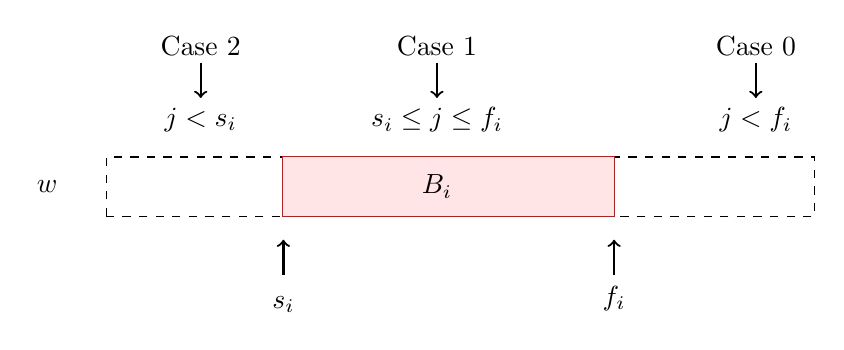
\begin{tikzpicture}[scale=1.5]
        % Main Rectangle w
        \draw[dashed] (0,0) rectangle (6,0.5);
        \node at (-0.5, 0.25) {\(w\)};

        % Smaller Rectangle 1 - Border color red
        \draw[draw=red, thick] (1.5,0) rectangle (4.3,0.5);
        
        \draw[->, thick] (1.5,-0.5) -- (1.5,-0.2);
        \node[align=center, below] at (1.5,-0.6) {\(s_{i}\)};
        \fill[red!10] (1.5,0) rectangle (4.3,0.5);
        \node at (2.8,0.25) {$B_{i}$};
        
        \draw[->, thick] (4.3,-0.5) -- (4.3,-0.2);
        
        \node at (4.3,-0.7) {$f_i$};
        
        
        \draw[->, thick] (5.5,1.3) -- (5.5,1);        
        \node[align=center, below] at (5.5,1) {\( j<f_i\)};
        \node[align=center, below] at (5.5,1.6) { \text{Case 0}};

        \draw[->, thick] (2.8,1.3) -- (2.8,1);        
        \node[align=center, below] at (2.8,1) {\( s_i \leq j \leq f_i\)};
        \node[align=center, below] at (2.8,1.6) {\text{Case 1}};

        \draw[->, thick] (0.8,1.3) -- (0.8,1);        
        \node[align=center, below] at (0.8,1) {\( j<s_i\)};
        \node[align=center, below] at (0.8,1.6) {\text{Case 2}};
        


    \end{tikzpicture}
    \caption{Compression for $w$ where $j$ is located.}
    \label{fig:case0}
\end{figure}


% So then, for case 0 $f_i<j$, it means that $s_i=s'_i$ and $f_i=f'_i$, LZ77 algorithm produces the exactly same result for $w[1,...,f_i]=w'[1,...,f_i]$, therefore. $B'_i$ is the only block that starts inside $B_i$, indeed, furthermore, $B_k=B'_k \forall k \leq i$.
% conclude that $f_i'\geq j$. When the case 1 holds, If $s_i\leq j\leq f_i$. We firstly have when $s_i=s'_i$, so that $B_k=B'_k \forall k \leq i-1$, this implies that $f_{i-1}=f'_{i-1}$. Hence $s_i=f_{i-1}+1 = f'_{i-1}+1 = s'_i$. We secondly have $f'_i\geq j$, so then, LZ77 compression only changes when a character is unknown for the string, thus, compression for $w'$ in the block $B'_i$ ends when $f_i=j$, moreover could be even greater, we never can finish before the index $j$ since compression up to $j$ is the same, so $|\mathcal{M}_i|= 1$ or $|\mathcal{M}_i|= 2$. Moreover, when $f'_{i+1}\geq f_i$, since $f_i\geq j$ we basically know that $f_i>f'_{i+1}$ but it does not matter how further $f'_{i+1}$ goes, because LZ77 compression guarantees that we can copy a substring that are previously encode. this automatically means that $|\mathcal{M}_i|= 2$ that is our important fact. On the other hand, analysis for case 2 relies when $j<s_i$ but based on LZ77 compression, when $j$ is placed before where the string for the block is copied over, it means that any place is located at compression for $w'$ adds at least 1 more block $B'_t$ that starts inside $B_k$ however since the condition holds we know that $f_i>f'_{i+1}$ therefore $|\mathcal{M}_i| \leq 2$.
% \end{proof}

% %%%%%%%%%%%%%%%%%%%%%%

% Let $t$ the maximum number of blocks after compressing $w'$ that \emph{Start Inside} $w$, since $w \sim w'$, then there is always a compression $(B'_1,...,B'_t)$ such as, WLOG $t'\geq t$ therefore, we defined $t'= \sum_{i=1}^{\infty}|\mathcal{M}_i|$, and $t= \sum_{i=1}^{\infty}|\mathcal{M}_i|$. These calculations are required for determine the quantity of blocks that \emph{Start Inside} either $B$ or $B'$ as a quantified property. Based on this reasoning and \defref{def:local_sensitivity} we introduce the difference to obtain Global Sensitivity, so then formally \claimref{claim:set:blocksm2:GS} as:
% %%%%%%%%%%%%%%%%%%%%%%%






% \lemblocknumupperbound

% \begin{proof}
%         If $i\in\B_2$ then either (1) $s_i\leq j\leq f_i$ or (2) $j-\ell_i < q_i \leq j$. When $j >f_i$, by LZ77 compression $B_i=B'_i$, thus $|\mathcal{M}_i|= 1$ and $i \in \mathcal{B_1}$.Hence, we have $s_i\leq j\leq f_i$ if $j\geq s_i$.
    
%     On the other hand, If $j<s_i$, then we want to show that $j-\ell_i<q_i\leq j$, i.e., $q_i\leq j < q_i+\ell_i$.
%     % \input{../Manuscript/figures/fig:claim9:case2}
%     Suppose for contradiction that $j\not\in[q_i,q_i+\ell_i-1]$.
%     Let $k$ be the smallest element in $\M_i$, i.e., $s_i\leq s_k'\leq f_i$ but $s_{k-1}'<s_i$.         
%     If $s_k'=f_i$, then if there is another $k'\in\M_i$ with $k'\neq k$, then by choice of $k$, we have $k<k'$ and therefore $s_{k'}'>f_k'>s_k'=f_i$. Hence, $|\M_i|= 1$ and $i\in\B_1$. Contradiction! It happens with any case for $j\not\in[q_i,q_i+\ell_i-1]$, since $i \in \B_2$. 
    
%     Now based on this, we are sure If $i_1,i_2\in\B_2$ then $(q_{i_1},\ell_{i_1})\neq(q_{i_2},\ell_{i_2})$. Since $i_1<i_2$ we then have $j<s_{i_1}<s_{i_2}$. Let $B_{i_1}=[q_{i_1},\ell_{i_1},c_{i_1}]$ and $B_{i_2}=[q_{i_2},\ell_{i_2},c_{i_2}]$ be  the blocks $B_{i_1}$ and $B_{i_2}$ of the LZ77 compression function $\compress:(\Sigma)^*\rightarrow(\Sigma')^*$ (Resp. w'). By intuition we know that there is no possibility to start in the same point for both Blocks $B_{i_1}$ and $B'_k$ after being read $j$ previously.
    

%     Finally Let $\B_2^\ell\coloneqq\{i\in\B_2:\ell_i=\ell\}$ and suppose that $s_{i^*}\leq j\leq f_{i^*}$ for some $i^*\in[t]$. Then $|\B_2^\ell|\leq\ell$ for all $\ell\neq \ell_{i^*}$, and $|\B_2^{\ell_{i^*}}|\leq\ell_{i^*}+1$. Furthermore, we observe that the constraint about length is: $\sum_{i\in\B_2} (\ell_i+1)\leq n,$ and $    \sum_\ell x_\ell'(\ell+1) < \sum_\ell x_\ell  (\ell+1) \leq n$. To find the threshold $z$, we observe that
% $\sum_{\ell=0}^z \ell(\ell+1) = \frac{1}{3}z(z+1)(z+2)\leq n,$
% which implies $z^3\leq 3n$ and $z\leq\sqrt[3]{3n}$. Setting this value of $z$, we have $t_2 \leq \frac{\sqrt[3]{9}}{2} n^{2/3} + \frac{\sqrt[3]{9}}{2} n^{1/3} + 1,$.
% \end{proof}

% The main result of this subsection is based on the analysis for upper bounding the global sensitivity, so then, in \secref{sec:upperbound} the goal is to provide the exact coefficient for the bound as is shown in the following theorem:




\section{Lower Bound for the Global Sensitivity of LZ77 Compression}\seclab{sec:lowerbound}

% =====

% \paragraph*{String Construction for the GS Lower Bound.}

% To prove the lower bound $\Omega(n^{2/3}\log^{1/3}n)$ for the global sensitivity of the LZ77 compression, we need to give example strings $w\sim w'$ of length $n$ that achieves $\left||\compress(w)|-|\compress(w')|\right|=\Omega(n^{2/3}\log^{1/3} n)$ (where $\compress$ denotes the LZ77 compression function) since this implies
% \begin{align*}
%     \mathtt{GS}_{\mathtt{Compress}} &= \max_{x \in \Sigma^n} \mathtt{LS}_{\mathtt{Compress}}(x)\\
%     &= \max_{x \in \Sigma^n}\max_{x' \in \Sigma^n:x\sim x'} \left| |\compress(x)| - |\compress(x')| \right|\\
%     &\geq \left||\compress(w)|-|\compress(w')|\right|\\
%     &=\Omega(n^{2/3}\log^{1/3} n).
% \end{align*}
% We give strings $w\sim w'$ that are carefully crafted such that $|w|=|w'|=\Theta(m^3\log m)$ for some integer $m>0$ and the number of type-2 blocks is $\Theta(m^2)$, which implies that $\GS_\compress=\Omega(m^2\log m) = \Omega(n^{2/3}\log^{1/3}n)$ where $n=\Theta(m^3\log m)$ denotes the length of strings. A core component of the string construction is to consider an \emph{injective encoding} of the number set $[m]$, which takes $\lceil\log m\rceil$ bits for each encoding, to ensure that each encoding is unique. This helps us count the number of type-2 blocks. However, having an injective encoding only does not fully resolve the issue 

% We overcome this bottleneck by \emph{repeating} each encoding twice.

% =====

In \secref{sec:upperbound}, we proved that the upper bound for the global sensitivity of the LZ77 compression algorithm $\compress$ is $O(n^{2/3}\log n)$ with window size $W=n$. One could ask if this is a tight bound, i.e., if we can prove the matching \emph{lower bound} for the global sensitivity of $\compress$ as well. This section proves the almost-matching lower bound up to a sub-logarithmic factor. In particular, we show that the global sensitivity of the LZ77 compression algorithm is $\Omega(n^{2/3}\log^{1/3} n)$. To prove the lower bound, we need to give example strings $w\sim w'$ of length $n$ that achieves $\left||\compress(w)|-|\compress(w')|\right|=\Omega(n^{2/3}\log^{1/3} n)$ since this implies $\GS_\compress=\max_{x \in \Sigma^n}\max_{x' \in \Sigma^n:x\sim x'} \left| |\compress(x)| - |\compress(x')| \right|\geq \left||\compress(w)|-|\compress(w')|\right|=\Omega(n^{2/3}\log^{1/3} n)$. 
% \begin{align*}
%     \mathtt{GS}_{\mathtt{Compress}} &= \max_{x \in \Sigma^n}\max_{x' \in \Sigma^n:x\sim x'} \left| |\compress(x)| - |\compress(x')| \right|\\
%     &\geq \left||\compress(w)|-|\compress(w')|\right|=\Omega(n^{2/3}\log^{1/3} n).
% \end{align*}
For the rest of \secref{sec:lowerbound}, we will give the construction of such example strings $w$ and $w'$.

\subsection{String Construction}

Consider an encoding function $\Enc:\mathbb{Z}\rightarrow\bin^*$ that maps integers to binary strings. Then for a positive integer $m\in\mathbb{Z}$, we have an injective encoding of the number set $\mathcal{S}\coloneqq\left\{0,1,\ldots, m\right\}$ using $\lceil\log m\rceil$ bits, i.e., $\Enc(i)\neq\Enc(j)$ if $i,j\in\mathcal{S}$ and $i\neq j$. For example, if $m=2^q-1$ for some positive integer $q$, we could encode the elements of $\S$ as follows: 
\[\Enc(0)=0^{\lceil\log m\rceil},\Enc(1)=0^{\lceil\log m\rceil-1}1,\Enc(2)=0^{\lceil\log m\rceil-2}10,\ldots,\Enc(m)=1^{\lceil\log m\rceil}.\] 
Now, consider a quinary alphabet $\Sigma=\{0,1,2,3,4\}$ and define a string
\[S_{\ell,u}\coloneqq\Enc(m-u+1)^2\circ\Enc(m-u+2)^2\circ\cdots\circ\Enc(m)^2\circ 2 \circ\Enc(m+1)^2\circ\cdots\circ\Enc(m-u+\ell)^2 \]
in $\Sigma^*$ for $2\leq\ell\leq m$ and $1\leq u\leq\ell-1$. 
Here, $(\cdot)^2$ denotes the concatenation of the string itself twice, i.e., $\Enc(\cdot)^2=\Enc(\cdot)\circ\Enc(\cdot)$. 
We define a procedure called $\QuinStr(m)$ which takes as input a positive integer $m\in\mathbb{Z}$ and outputs two quinary strings as follows.

\begin{tcolorbox}[breakable,enhanced,title={The Construction of Two Quinary Strings $\QuinStr(m)$.}]
    \begin{enumerate}
        \item The algorithm computes two quinary strings $S_w$ and $S_{w'}$ where
        \begin{align*}
            S_w &\coloneqq\Enc(1)^2\circ\cdots\circ\Enc(m)^2\circ 2 \circ\Enc(m+1)^2\circ\cdots\circ\Enc(2m)^2\circ 4,\text{ and}\\
            S_{w'} &\coloneqq\Enc(1)^2\circ\cdots\circ\Enc(m)^2\circ 3 \circ\Enc(m+1)^2\circ\cdots\circ\Enc(2m)^2\circ 4.
        \end{align*}
        \item Then it computes two quinary strings $w,w'$ defined as $w\coloneqq S_w\circ S$ and $w'\coloneqq S_{w'}\circ S$, where
        \[S = S_{2,1} \circ 4 \circ S_{3,2} \circ 4 \circ S_{3,1} \circ 4 \circ \ldots \circ S_{m,m-1} \circ 4 \circ \ldots \circ S_{m,1}\circ 4.\]
        \item Output $(w,w')$.
    \end{enumerate}
\end{tcolorbox}

\claimref{claim:length} tells us that the strings $w$ and $w'$ outputted by the procedure $\QuinStr(m)$ has equal length $\Theta(m^3\log m)$. Since the proof is elementary, we defer the proof of \claimref{claim:length} to \appref{app:missingprooflowerbound}.

\newcommand{\claimlength}{
Let $m\in\mathbb{N}$ and $(w,w')\gets\QuinStr(m)$. Then $|w|=|w'|=\Theta(m^3\log m)$. In particular, for $m\geq 4$, $\frac{2}{3}m^3\lceil\log m\rceil< |w|=|w'|< m^3\lceil\log m\rceil$.
}
\begin{claim}\claimlab{claim:length}
\claimlength
\end{claim}

\subsection{Analyzing the Sensitivity of $\QuinStr(m)$}

A central step in our sensitivity analysis for $\QuinStr(m)$ is precisely counting the type-2 blocks produced by the LZ77 compression scheme, as we observed in \secref{sec:upperbound}. \lemref{lem:gs} shows that for $(w,w')\gets\QuinStr(m)$, we have $|\B_2|=\frac{(m-1)m}{2}-(\lfloor\frac{m}{2}\rfloor-1)$. Intuitively, we first show that for $w=S_w\circ S$, there is no type-2 block for the blocks compressing $S_w$. Then the main insight is that we carefully crafted strings $w$ and $w'$ such that the marker symbol `4' becomes the endpoint for each block in $\compress(w)$ for the tail part $S$ of $w=S_w\circ S$. By repeating each encoding twice, we can ensure that most of the occurrences of $S_{\ell,u}\circ 4$ yield type-2 blocks, with an edge case (addressed in \claimref{claim:repeat}) that makes the block in $\B_1$ but this happens for only about $m/2$ blocks. Consequently, despite these few exceptions, the overall count of type-2 blocks remains quadratic in $m$.

\newcommand{\lemGS}{
Let $m\in\mathbb{N}$ and $(w,w')\gets\QuinStr(m)$ and let $\compress:\Sigma^*\rightarrow(\Sigma')^*$ be the LZ77 compression algorithm. Let $(B_1,\ldots,B_t)\gets\compress(w)$ and $(B'_1,\ldots,B'_{t'})\gets\compress(w')$. Then $|\B_0| = 0$ and $|\B_2| = \frac{(m-1)m}{2}-(\lfloor\frac{m}{2}\rfloor-1)$.
}
\begin{lemma}\lemlab{lem:gs}
    \lemGS
\end{lemma}

\begin{proof}
Recall that $w = S_w \circ S$ and $w' = S_{w'} \circ S$, where
\begin{itemize}
    \item $S_w =\Enc(1)^2\circ\cdots\circ\Enc(m)^2\circ 2 \circ\Enc(m+1)^2\circ\cdots\circ\Enc(2m)^2\circ 4$,
    \item $S_{w'}=\Enc(1)^2\circ\cdots\circ\Enc(m)^2\circ 3 \circ\Enc(m+1)^2\circ\cdots\circ\Enc(2m)^2\circ 4$, and
    \item $S=S_{2,1} \circ 4 \circ S_{3,2} \circ 4 \circ S_{3,1} \circ 4 \circ \ldots \circ S_{m,m-1} \circ 4 \circ \ldots \circ S_{m,1}\circ 4$, where
    \item $S_{\ell,u}\coloneqq\Enc(m-u+1)^2\circ\Enc(m-u+2)^2\circ\cdots\circ\Enc(m)^2\circ 2 \circ\Enc(m+1)^2\circ\cdots\circ\Enc(m-u+\ell)^2$ for $2\leq\ell\leq m$ and $1\leq u\leq \ell-1$.
\end{itemize}
We first observe that $w\sim w'$. Define $S_w^F\coloneqq \Enc(1)^2\circ\cdots\circ\Enc(m)^2\circ 2$ (resp. $S_{w'}^F\coloneqq \Enc(1)^2\circ\cdots\circ\Enc(m)^2\circ 3$) to be the first-half substring of $S_w$ (resp. of $S_{w'}$), and $S_w^L=S_{w'}^L\coloneqq \Enc(m+1)^2\circ\cdots\circ\Enc(2m)^2\circ 4$ to be the last-half substring of $S_w$ (or $S_{w'}$ since they are indeed identical). 
It is useful to define a notation $\str(B_k)$ for a block $B_k$, which denotes the substring of $w$ represented by the block $B_k$, i.e., for $B_k=[q_k,\ell_k,c_k]$, $\str(B_k)\coloneqq w[q_k,q_k+\ell_k-1]\circ c_k$. 

Let $B_{i_1}$ be the first block such that $S_w^F$ becomes a substring of $\str(B_1)\circ\str(B_2)\circ\ldots\circ\str(B_{i_1})$, and similarly, let $B'_{i'_1}$ be the first block such that $S_{w'}^F$ becomes a substring of $\str(B'_1)\circ\str(B'_2)\circ\ldots\circ\str(B'_{i'_1})$. Then we observe the following:
\begin{enumerate}
    \item $B_{i_1}=[q_{i_1},\ell_{i_1},2]$, i.e., $\str(B_{i_1})$ ends with $2$ (which is the last character in $S_w^F$), since $2$ never showed up before as all the encodings are binary strings, it has to be added to the dictionary as a new character,
    \item $B_i=B_i'$ for all $i\in[i_1-1]$, as we are compressing the identical strings until we see $2$ in $S_w^F$ (and $3$ in $S_{w'}^F$), and
    \item $i_1=i_1'$ and $B'_{i_1}=[q_{i_1},\ell_{i_1},3]$, since two strings $S_w^F$ and $S_{w'}^F$ are identical except for the very last character.\label{item:2}
\end{enumerate}

Now let $B_{i_2}$ be the first block such that $S_w^L$ becomes a substring of $\str(B_{i_1+1})\circ\str(B_{i_1+2})\circ\ldots\circ\str(B_{i_2})$, and similarly, let $B'_{i'_2}$ be the first block such that $S_{w'}^L$ becomes a substring of $\str(B'_{i_1+1})\circ\str(B'_{i_1+2})\circ\ldots\circ\str(B'_{i'_2})$. Then we observe the following:
\begin{enumerate}
\setcounter{enumi}{3}
    \item $i_2=i_2'$ and $B_i=B_i'$ for all $i\in[i_1+1,i_2]$, since $i_1=i_1'$ from observation \ref{item:2} and we have $S_w^L=S_{w'}^L$ while they do not contain $2$ or $3$, and
    \item $B_{i_2}=[q_{i_2},\ell_{i_2},4]$, since $4$ never showed up before in our compression.
\end{enumerate}

From the observations above, we have that $B_i\in\B_1$ for all $i\in[i_2]$. 
Now we are left with the blocks $(B_{i_2+1},\ldots,B_t)$ compressing the last part $S$ of $w$ and the blocks $(B'_{i_2+1},\ldots,B'_{t'})$ compressing the last part $S$ of $w'$. For the blocks $(B_{i_2+1},\ldots,B_t)$, we observe that each block ends at the next `$4$' because each $S_{\ell,u}$ (for $2\leq\ell\leq m$ and $1\leq u\leq \ell-1$) is contained in the former part of $w$ (which was $S_w$) but $4$ only shows up in $S_w$ followed by $\Enc(2m)^2$ while $S_{\ell,u}$ cannot contain $\Enc(2m)$. Hence, we observe the following:
\begin{enumerate}
\setcounter{enumi}{5}
    \item $\str(B_{i_2+1})=S_{2,1}\circ 4,\str(B_{i_2+2})=S_{3,2}\circ 4$,  and so on.
    \item In general, $\str\left(B_{i_2+\frac{(\ell-2)(\ell-1)}{2}+(\ell-t)}\right)=S_{\ell,u}\circ 4$, for $2\leq\ell\leq m$ and $1\leq u\leq \ell-1$. This indeed covers all the blocks from $B_{i_2+1},\ldots,B_t$ (See \claimref{claim:inj} and observation \ref{item:8}).
    \item Furthermore, we can observe that $t= i_2 + (1+2+\ldots+(m-1)) = i_2 + \frac{(m-1)m}{2}$.\label{item:8}
\end{enumerate}

\newcommand{\felluinjective}{
For any integer $m\geq 2$, the function $f(\ell,u)\coloneqq\frac{(\ell-2)(\ell-1)}{2}+(\ell-u)$ defined over integers $\ell$ and $u$ such that $2\leq \ell\leq m$ and $1\leq u\leq \ell-1$ is injective, and its range is $[\frac{(m-1)m}{2}]$.
}
\begin{claim}\claimlab{claim:inj}
\felluinjective
\end{claim}

The proof of \claimref{claim:inj} is elementary by induction on $m$, and hence, we defer the proof to \appref{app:missingprooflowerbound}. What we are interested in is whether each $B_i$, for $i_2+1\leq i\leq t$, belongs to $\B_0$, $\B_1$, or $\B_2$. In \claimref{claim:blocks}, we prove that the blocks are mostly in $\B_2$ and the rest of the blocks are in $\B_1$, meaning that $\B_0=\emptyset$. In particular, we prove that for $2\leq\ell\leq m$ and $1\leq u\leq\ell-1$, $B_{i_2+\frac{(\ell-2)(\ell-1)}{2}+(\ell-u)}\in\B_1$ if and only if all of these conditions hold: (1) $\ell>2$, (2) $\ell$ is even, and (3) $u=\ell/2$. 

\begin{claim}\claimlab{claim:blocks}
For $2\leq\ell\leq m$ and $1\leq u\leq \ell-1$, $B_{i_2+\frac{(\ell-2)(\ell-1)}{2}+(\ell-u)}\in\B_1$ if and only if $\ell>2, 2\mid\ell$, and $u=\ell/2$; otherwise $B_{i_2+\frac{(\ell-2)(\ell-1)}{2}+(\ell-u)}\in\B_2$.
%For $\ell'\in\left[\lfloor\frac{m}{2}\rfloor\right]$, $B_{i_2+(\ell'-1)(2\ell'-1)+\ell'}\in\B_1$ and 
\end{claim}

We will give the proof of \claimref{claim:blocks} below and finish the proof of \lemref{lem:gs} first for readability. By \claimref{claim:blocks}, since there are only $\lfloor\frac{m}{2}\rfloor-1$ of such pairs of $(\ell,u)$, we observe that $|\B_2|=\frac{(m-1)m}{2}-(\lfloor\frac{m}{2}\rfloor-1)$. Since we have that $B_i\in\B_1$ for all $i\in[i_2]$, we have $\B_0=\emptyset$ and therefore $|\B_0|=0$. This completes the proof of \lemref{lem:gs}.
\end{proof}

\begin{proofof}{\claimref{claim:blocks}}
Recall that $S=S_{2,1}\circ4\circ S_{3,2}\circ4\circ S_{3,1}\circ4\circ\ldots\circ S_{m,m-1}\circ4\circ\ldots\circ S_{m,1}\circ4$ and $\str(B_{i_2+1})=S_{2,1}\circ4$, $\str(B_{i_2+2})=S_{3,2}\circ4$, $\str(B_{i_2+3})=S_{3,1}\circ4,\ldots,\str(B_t)=S_{m,1}\circ4$. 
For each $S_{\ell,u}$, we observe that $S_{\ell,u}$ is \emph{not} a substring of $S_{w'}$. Hence, we see that each block $B_i$ (for $i_2+1\leq i\leq t$) is roughly split into two blocks for the blocks of $\compress(w')$ unless it could copy beyond the character $4$. To observe the cases when this happens,
for each $S_{\ell,u}$, it is helpful to define:
\begin{itemize}
    \item $S_{\ell,u}^F\coloneqq\Enc(m-u+1)^2$ denotes the very first encoding concatenation that shows in $S_{\ell,u}$, 
    \item $S_{\ell,u}^{F,(1/2)}\coloneqq\Enc(m-u+1)$ denotes the very first encoding in $S_{\ell,u}$ (i.e., half of $S_{\ell,u}^F$),
    \item $S_{\ell,u}^L\coloneqq\Enc(m-u+\ell)^2$ denotes the very last encoding concatenation that shows in $S_{\ell,u}$, and
    \item For $k>u$, $S_{\ell,u}^{(k)}\coloneqq\Enc(m-u+1)^2\circ\Enc(m-u+2)^2\circ\ldots\circ\Enc(m)^2\circ2\circ\Enc(m+1)^2\circ\ldots\circ\Enc(m-u+k)^2$ denotes the first $k$ encoding concatenations that shows in $S_{\ell,u}$.
\end{itemize}
Then we observe the following claims. Since proofs of \claimref{claim:notrepeat} and \claimref{claim:repeat} are elementary, we defer the proofs to \appref{app:missingprooflowerbound}.

\begin{claim}\claimlab{claim:notrepeat}
$S_{\ell,u}^L\circ4\circ S_{\ell,u-1}^F$ does not repeat for different $\ell$ and $u$ such that $3\leq\ell\leq m$ and $2\leq u\leq\ell-1$.
\end{claim}

\claimref{claim:notrepeat} tells us that, due to the injectivity of the encoding, any block in $\compress(w')$ containing a portion of $S_{\ell,u}^L$ along with the delimiter `4' must finish at $S_{\ell,u}^{F,(1/2)}$ in the worst case. In particular, note that $S_{\ell,u}^L=\Enc(m-u+\ell)^2=S_{\ell+1,u+1}^L$ for $3\leq \ell<m$ and $2\leq u<\ell-1$. Moreover, we have $S_{\ell,u-1}^{F,(1/2)}=\Enc(m-u+2)$ and $S_{\ell+1,u}^{F,(1/2)}=\Enc(m-u+1)$, which can agree on all but the final bit (e.g., $S_{\ell,u-1}^{F,(1/2)}=00\cdots00$ and $S_{\ell+1,u}^{F,(1/2)}=00\cdots01$). Without the repetition of each encoding, a block might incorporate nearly the entire $S_{\ell+1,u}^{F,(1/2)}$ except for the last bit. Consequently, by having this last bit as a new character, $S_{\ell,u-1}\circ4$ would be placed in $\B_1$. Repeating the encoding twice eliminates this possibility and we can ensure that the scenario described in \claimref{claim:repeat} is the only case where type-1 blocks would occur. Again, see \appref{app:missingprooflowerbound} for the proof of \claimref{claim:repeat}.


\begin{claim}\claimlab{claim:repeat}
For $2\leq\ell\leq\lfloor\frac{m}{2}\rfloor-1$, $S_{\ell,1}^L\circ4\circ S_{\ell+1,\ell}$ repeats at $S_{2\ell,\ell+1}^L\circ4\circ S_{2\ell,\ell}^{(\ell+1)}$.
\end{claim}

Let's go back to the proof of \claimref{claim:blocks}. By \claimref{claim:repeat}, we can see that the block of the form $B_{i_2+\frac{(2\ell-2)(2\ell-1)}{2}+(2\ell-\ell)}$ which satisfies
\[\str\left(B_{i_2+\frac{(2\ell-2)(2\ell-1)}{2}+(2\ell-\ell)}\right)=S_{2\ell,\ell}\circ4,\]
is in $\B_1$, and all of the other blocks beyond $B_{i_2}$ are in $\B_2$. This completes the proof of \claimref{claim:blocks}.
% We first observe the following.
% Now, let's analyze the blocks $(B'_{i_2+1},\ldots,B'_{i'_3})$. Consider $B'_{i_2+1}$ first as a warmup. Recall that $\str(B_{i_2+1})=S_{2,1}\circ 4$ because $S_{2,1}=\Enc(m)^2\circ 2\circ \Enc(m+1)^2$ was a substring of $S_w$, but this is \emph{not} the case for $w'$ since we replaced $2$ with $3$ in $S_{w'}$. This observation implies that $\str(B'_{i_2+1})=\Enc(m)^2\circ 2$ (which is the substring of $S_{2,1}$) since $\Enc(m)^2$ was contained in $S_{w'}$ and it is indeed the longest substring you could copy from the prior substring since $2$ never showed up in $w'$.
% Next, consider the next block $B'_{i_2+2}$. It is easy to see that $\str(B'_{i_2+2})=\Enc(m+1)^2\circ 4$ because $\Enc(m+1)^2$ is a substring of $S_{w'}$ and $4$ only showed up once in a prior substring, followed by $\Enc(2m)^2$ (in $S_{w'}\circ 4$). With a similar argument, we observe that $\str(B'_{i_2+3})=\Enc(m-1)^2\circ\Enc(m)^2\circ 2$ (which is a substring of $S_{3,2}$). Now for the block $B'_{i_2+4}$, one might think that $\str(B'_{i_2+4})=\Enc(m+1)^2\circ 4\circ c'_{i_2+4}$ where $c'_{i_2+4}$ is the first character in $\Enc(m)$ (since $S_{3,1}$ starts with $\Enc(m)^2$) since it seems to be the case that $\Enc(m+1)^2\circ 4$ is the longest substring of $S_{w'}\circ 4 \circ S_{2,1}\circ 4\circ \Enc(m-1)^2\circ\Enc(m)^2\circ 2$
\end{proofof}

Taken altogether, we can lower bound the global sensitivity of the LZ77 compression scheme as stated in \thmref{thm:lowerbound} below.

\begin{theorem}\thmlab{thm:lowerbound}
Let $\compress:\Sigma^*\rightarrow\Sigma'^*$ be the LZ77 compression function. Then $\mathtt{GS}_\compress\geq 4^{-1/3}\cdot n^{2/3}\log^{1/3}n=\Omega(n^{2/3}\log^{1/3}n)$. 
\end{theorem}

\begin{proof}
Let $(w,w')\gets\QuinStr(m)$ and let $|w|=|w'|=n$. By \claimref{claim:length}, we have $|w|=|w'|=\Theta(m^3\log m)$ and therefore $n=\Theta(m^3\log m)$. Furthermore, \claimref{claim:length} tells us that there exists some $\alpha$ with $\frac{2}{3}\leq\alpha\leq 1$ such that $n=\alpha m^3\log m$.  
Now let $(B_1,\ldots,B_t)\gets\compress(w)$ and $(B'_1,\ldots,B'_{t'})\gets\compress(w')$.
Recall that if we look at the proof of \claimref{claim:set:blocksm2:GS}, it tells us that $t'-t=|\B_2|-|\B_0|$. From \lemref{lem:gs}, we have $|\B_0|=0$ and $|\B_2|=\frac{(m-1)m}{2}-(\lfloor\frac{m}{2}\rfloor-1)$, which implies that $t'-t=\frac{(m-1)m}{2}-(\lfloor\frac{m}{2}\rfloor-1)$. We know $|\compress(w)|=t(2\lceil\log n\rceil+\lceil\log|\Sigma|\rceil)$ and $|\compress(w')|=t'(2\lceil\log n\rceil+\lceil\log|\Sigma|\rceil)$, we have
\begin{align*}
   \mathtt{GS}_{\mathtt{Compress}} & \leq  \left||\compress(w)|-|\compress(w')|\right|  
   = |t-t'|\left(2\lceil\log n\rceil+\lceil\log|\Sigma|\rceil\right) \\
    &= |t-t'|\left(2\left\lceil\log (\alpha m^3\log m)\right\rceil+\lceil\log|\Sigma|\rceil\right) 
    %\geq \left[\frac{(m-1)m}{2}-\left(\left\lfloor\frac{m}{2}\right\rfloor-1\right)\right]\cdot2\log(\alpha m^3\log m)\\
    \geq \frac{m^2}{4}\cdot 4\log m = m^2\log m \ .
\end{align*}
% \begin{align*} backup for full version
%     \left||\compress(w)|-|\compress(w')|\right| &= |t-t'|\left(2\lceil\log n\rceil+\lceil\log|\Sigma|\rceil\right) \\
%     &= |t-t'|\left(2\left\lceil\log (\alpha m^3\log m)\right\rceil+\lceil\log|\Sigma|\rceil\right)\\
%     &\geq \left[\frac{(m-1)m}{2}-\left(\left\lfloor\frac{m}{2}\right\rfloor-1\right)\right]\cdot2\log(\alpha m^3\log m)\\
%     &\geq \left(\frac{m^2}{2}-m\right)\cdot 4\log m\\
%     &\geq \frac{m^2}{4}\cdot 4\log m = m^2\log m,
% \end{align*}
%which implies that
%\begin{align*}
 %   \mathtt{GS}_{\mathtt{Compress}} &= \max_{x \in \Sigma^n}\max_{x' \in \Sigma^n:x\sim x'} \left| |\compress(x)| - |\compress(x')| \right|\\
 %   &\geq \left||\compress(w)|-|\compress(w')|\right|\\
  %  &= m^2\log m.
%\end{align*}
Furthermore, since we have $n=\alpha m^3\log m$ for some $\frac{2}{3}\leq\alpha\leq 1$, we observe that
\begin{align*}
    m^2\log m &= m^2\cdot\frac{n}{\alpha m^3}= \frac{n}{\alpha}\cdot\frac{1}{m} = \frac{n}{\alpha}\cdot\frac{\alpha^{1/3}\cdot\log^{1/3}m}{n^{1/3}}
    \geq \left(\frac{n}{\alpha}\right)^{2/3}\cdot 4^{-1/3}\cdot\log^{1/3}n \\
    &\geq 4^{-1/3}\cdot n^{2/3}\log^{1/3}n,
\end{align*}
% \begin{align*} backup for full version
%     m^2\log m &= m^2\cdot\frac{n}{\alpha m^3}\\
%     &= \frac{n}{\alpha}\cdot\frac{1}{m}\\
%     &= \frac{n}{\alpha}\cdot\frac{\alpha^{1/3}\cdot\log^{1/3}m}{n^{1/3}}\\
%     &= \left(\frac{n}{\alpha}\right)^{2/3}\cdot\log^{1/3}m\\
%     &\geq \left(\frac{n}{\alpha}\right)^{2/3}\cdot 4^{-1/3}\cdot\log^{1/3}n\\
%     &\geq 4^{-1/3}\cdot n^{2/3}\log^{1/3}n,
% \end{align*}
where the first inequality comes from the observation $\log n = \log\alpha + 3\log m + \log\log m\leq 4\log m$ and the second inequality comes from $(1/\alpha)\geq 1$. Hence,
\begin{align*}
    \mathtt{GS}_{\mathtt{Compress}} &\geq m^2\log m \geq 4^{-1/3}\cdot n^{2/3}\log^{1/3}n,
\end{align*}
% Since we know $\frac{2}{3}\cdot m^3\log m\leq n\leq m^3\log m$ from \claimref{claim:length}, we observe that 
% \begin{align*}
%     m^2\log m &= \frac{1}{m}\cdot m^3\log m\\
%     &\geq \frac{1}{m}\cdot n\\
%     &\geq \sqrt[3]{\frac{2}{3}}\cdot n^{-1/3}\cdot\left(\log^{1/3}m\right)\cdot n\\
%     &\geq \sqrt[3]{\frac{2}{3}}\cdot n^{-1/3}\cdot\left(\sqrt[3]{\frac{1}{6}}\cdot\log^{1/3}n\right)\cdot n\\
%     &= \sqrt[3]{\frac{1}{9}}\cdot n^{2/3}\log^{1/3}n,
% \end{align*}
% where the third inequality is achieved by the observation that $3\log m\geq \log n - \log\log m \geq \frac{\log n}{2}$, since $\log m\leq \sqrt{n}$.
% Hence,
% \begin{align*}
%     \mathtt{GS}_{\mathtt{Compress}} &\geq m^2\log m\\
%     &\geq \sqrt[3]{\frac{1}{9}}\cdot n^{2/3}\log^{1/3}n,
% \end{align*}
which completes the proof.
\end{proof}

\subsection{Robustness of CDDI}
Since the CDDI is calculated by comparing the concordant and discordant pairs of two different constraint orders, there are usually multiple constraint orders sharing the same CDDI value. Therefore, we conduct a testing experiment to assess whether the LLM exhibits significant fluctuations across different constraint orders with the same CDDI value. Specifically, we set the CDDI to -0.05, a value that includes the most constraint orders in our setting, and conduct single-round inference for 3 times. The experiment results are shown in Tab~\ref{tab:sensitivity}. We calculate the P-value of the data, finding that the P-value is much larger than 0.05. This indicates that the fluctuation of LLM's performance is negligible among different constraint orders in the same CDDI value.




\section{Explanation Study}

\begin{figure*}[t] 
    \centering
        \includegraphics[width=1\textwidth]{position_scores.pdf}
    % \captionsetup{font={small}} 
    \caption{(a) The importance weights assigned by the LLM when handling constraints in different positions. (b) The total importance weights which designated to the constraint part in the multi-constraint instructions among three different constraint distributions.}
    \label{fig:position_score}
\end{figure*}


\begin{figure}[t] 
    \centering
        \includegraphics[width=0.48\textwidth]{types_scores.pdf}
    % \captionsetup{font={small}} 
    \caption{The importance weights across different types of constraint in three different constraint distributions.}
    \label{fig:type_score}
\end{figure}







\subsection{Explanation Metric}
To make an explanation for the influence brought by the constraints of different orders, we make an explanation study on where the LLMs mainly focus when handling multi-constraint instructions via a feature attribution-based explanation method~\cite{li2016visualizing, wu2020perturbed}. Specifically, we leverage the importance of the input tokens to measure the LLMs' attention to them. To obtain the importance of a specific instruction token $t_x$ to a response token $t_y$, we calculate the confidence change after the removal of the $t_x$, as formulated below:
\begin{equation}
    \label{eq6}
    I_{t_x,t_y}=p(t_y|Z_y)-p(t_y|Z_{y,/t_x}),
\end{equation}
where $p(\cdot|\cdot)$ is the conditional probability produced by the LLM $f$, $Z_y$ is the tokens before the $t_y$ and $Z_{y,/t_x}$ is the tokens of $Z_y$ after removing the token $t_x$. To reduce the computation, we approximate the $I_{t_x,t_y}$ with the first-order gradient $\frac{\partial f\left(t_y \mid Z_y\right)}{\partial \mathbf{E}\left[t_x\right]}$ ~\cite{wu2023language}, where $\mathbf{E}\left[t_x\right]$ is the token embedding of $t_x$. We normalize the importance $I_{t_x,t_y}$ and obtain the standard importance $S_{t_x,t_y}$ with the formula:
\begin{equation}
    \label{eq7}
    S_{t_x,t_y}= \frac{L\times I_{t_x,t_y}}{{\max_{i=1}^{N_{X}}}I_{t_i,t_y}},
\end{equation}
where $N_X$ is the number of instruction tokens and $L$ is a hyper-parameter which helps to filter the noise brought by the first-order approximation. To visualize the LLMs' attention to different constraints, we calculate the importance weight of a specific constraint $C_x$ to the final response $Y$ with the formula:
\begin{equation}
    \label{eq8}
    S_{C_x,Y}=\frac{1}{N_Y}\sum_{t_y\in Y}\sum_{t_x\in C_x}S_{t_x,t_y},
\end{equation}
where $N_Y$ is the number of response tokens.







\subsection{Experiment Set-up}
We conduct our explanation study on the LLaMA3-8B-Instruct model. We set the hyper-parameter $L$ to 10 in Eq.(\ref{eq7}) and select three most typical difficulty distributions: hard-to-easy (indicated by CDDI=1), easy-to-hard (indicated by CDDI=-1) and random (indicated by CDDI=-0.05) to conduct our experiments. We randomly sample 200 instances from the corresponding data which fall in the required CDDI value in the probing task to serve as the dataset.







\subsection{Results}
\paragraph*{Hard-to-easy constraint order induces the LLM to pay more attention to the constraint part in the multi-constraint instructions.} We visualize the importance weights of the model on the constraints in different positions. As shown in Fig.~\ref{fig:position_score} (a), in the multi-constraint instruction following, the model's attention on different positions varies with changes in the constraint orders. Specifically, when the constraints are randomly distributed across different positions (represented by CDDI=-0.05), the model assigns similar attention to all positions. As the constraint order becomes more structured (represented by CDDI=-1 and CDDI=1), the model's attention neither exhibits the “lost in the middle” phenomenon observed in long-context processing~\cite{liu2024lost}, nor a simply sequential distribution, but follows an iterative, laddered order. Then, in Fig.~\ref{fig:position_score} (b), we present the total importance weight the model assigns to the constraint part. We observe that the “hard-to-easy” constraint order attracts the most attention from the model towards the constraint part, which provides an explanation for the superiority of this constraint order.

\paragraph*{The LLM's performance on various constraints is strongly correlated with its attention patterns.} The importance weights of the model on different types of constraints are presented in Fig.~\ref{fig:type_score}. Among the three distinct difficulty distributions, the “hard-to-easy” (represented by CDDI = 1) assigns the highest importance weights to various types of constraints except for the Content and Startend. It is worth noting that this is exactly in accord with quantitative results in Tab.~\ref{tab:main}, i.e., as the CDDI value increases, the model's performance on the Content and Startend constraints shows a decreasing trend instead. Overall, the results show that the model's accuracy in following a specific type of constraint is strongly correlated with the attention assigned to it by the model. \label{sec:experiment2}

\section{Conclusion}

In this paper, we systematically investigate the position bias problem in the multi-constraint instruction following. To quantitatively measure the disparity of constraint order, we propose a novel Difficulty Distribution Index (CDDI). Based on the CDDI, we design a probing task. First, we construct a large number of instructions consisting of different constraint orders. Then, we conduct experiments in two distinct scenarios. Extensive results reveal a clear preference of LLMs for ``hard-to-easy'' constraint orders. To further explore this, we conduct an explanation study. We visualize the importance of different constraints located in different positions and demonstrate the strong correlation between the model's attention distribution and its performance.

\section{Limitations}

Our work mainly focuses on the position bias problem in the multi-constraint instruction following. We make a quantitative analysis of the influence brought by different constraint orders in the instructions. However, there are still some limitations. The constraints in our work are usually parallel to each other, which means the order change will not affect the semantic meaning of the instructions. The position bias problem for for those sequential constraints need to be further explored. Moreover, we only investigate the phenomenon of position bias in existing LLM without offering a solution. In further work, we will conduct a further probing task in sequential constraints to improve the generalization of our findings.

% \section*{Acknowledgments}

% This document has been adapted
% by St

% Bibliography entries for the entire Anthology, followed by custom entries
%\bibliography{anthology,custom}
% Custom bibliography entries only
\bibliography{acl_latex}

\appendix

\section{Appendix}

\clearpage
\appendix
\onecolumn
\section{Implementation Details}
\subsection{Token-aware Preference Data Construction}
\label{sec:impl}
For all models that used for preference data construction, we adopt the following prompts presented in Figure \ref{fig: prompt-decom}, \ref{fig: prompt-selfinst}, \ref{fig: prompt-recomb}, \ref{fig: prompt-sub}, \ref{fig: prompt-neg} and \ref{fig: prompt-sub}. We set the temperate as 0.5 for all steps to ensure diversity. To ensure the data quality, we filter instructions with less than three constraints and more than ten constraints. We also filter preference pairs with the same chosen and rejected responses. 

For constraint dropout, we set the dropout ratio $\alpha$ to 0.3 to ensure that negative examples are sufficiently negative, meanwhile not deviate too much from the positive sample. We avoid dropout on the first constraint, as it often establishes the foundation for the task, and dropping the first one would make the recombined instruction overly biased.

\subsection{Token-aware Preference Optimization}
\label{sec:impl-dpo}
Our experiments are based on Llama-Factory \cite{zheng2024llamafactory}, and we trained all models on 8 A100-80GB SXM GPUs. The \texttt{per\_device\_train\_batch\_size} was set to 1, \texttt{gradient\_accumulation\_steps} to 8, leading to an overal batch size as 64, and we used bfloat16 precision. The learning rate is set as 1e-06 with cosine decay,and each model is trained with 2 epochs. We set $\beta$ to 0.2 for all DPO-based experiments, $\beta$ as 3.0 and $\gamma$ as 1.0 for all SimPO-based experiments, $\beta$ as 1.0 for all IPO-based methods referring to the settings of \citet{meng2024simpo}. All of the final loss includes 0.1x of the SFT loss.

\section{The Influence of Noising Scheme}
\label{app:noising}

Previous work has proposed various noising strategies in contrastive training \cite{lai-etal-2021-saliency-based}. While we leverage Constraint-Dropout for negative sample generation, to make a fair comparison with other strategies, we implement the following strategies: 1) Constraint-Negate: Leverage the model to generate an opposite constraint. 2) Constraint-Substitute: Substitute the constraint with an unrelated constraint.

\begin{figure}[h]
\centering
\includegraphics[width=0.6\linewidth]{figures/drop_ratio.png}
\caption{The variation of results on CFBench and AlpacaEval2 with different dropout ratios.}
\label{fig:drop_ratio}
\end{figure}

As shown in Table \ref{tab:detail-noising}, both the negation and substitution applied on the constraints would lead to performance degradation. After a thoroughly inspect of the derived data, we realize that instructions derived from both dropout and negation would lead to instructions too far from the positive instruction, therefore the derived negative response would also deviate too much from the original instruction. An effective negative sample should fulfill both negativity, consistency and contrastiveness, and constrait-dropout is a simple yet effective method to achieve this goal.

We also provide the variation of the results on CF-Bench and AlpacaEval2 with different constraint dropout ratios. As shown in Figure \ref{fig:drop_ratio}, with the dropout ratio increased from 0.1 to 0.5, the results on CF-Bench firstly increases and then slightly decreases. On the other hand, the results on AlpacaEval2 declines a lot with a higher dropout ratio. This denotes that a suboptimal droout ratio is essential for the balance between complex instruction and general instruction following abilities, with lower ratio may decrease the effectiveness of general instruction alignment, while higher ratio may be harmful for complex instruction alignment. Finally, we set the constraint dropout ratio as 0.3 in all experiments.

\begin{table*}[tt]
\centering
\resizebox{1.0\textwidth}{!}{
\begin{tabular}{cc|ccccc|ccccc}
\toprule
\multirow{3}{*}{\textbf{Scenario}} & \multirow{3}{*}{\textbf{Method}} & \multicolumn{5}{c|}{\textbf{Meta-LLaMA-3-8B-Instruct}}                                    & \multicolumn{5}{c}{\textbf{Qwen-2-7B-Instruct}}                                          \\
                                   &                                  & \multicolumn{3}{c}{\textbf{CF-Bench}}         & \multicolumn{2}{c|}{\textbf{AlpacaEval2}} & \multicolumn{3}{c}{\textbf{CF-Bench}}         & \multicolumn{2}{c}{\textbf{AlpacaEval2}} \\
                                   &                                  & \textbf{CSR}  & \textbf{ISR}  & \textbf{PSR}  & \textbf{LC\%}      & \textbf{Avg.Len}     & \textbf{CSR}  & \textbf{ISR}  & \textbf{PSR}  & \textbf{LC\%}      & \textbf{Avg.Len}    \\ \midrule
\multirow{6}{*}{PreInst}           & baseline                         & 0.64          & 0.24          & 0.34          & 21.07              & 1702                 & 0.74          & 0.36          & 0.49          & 15.53              & 1688                \\ \cline{2-12} 
                                   & Constraint-Drop               & \textbf{0.71} & \textbf{0.34} & \textbf{0.45} & \textbf{23.43}     & 1682           & \textbf{0.79} & \textbf{0.43}  & \textbf{0.54}          & \textbf{19.31}     & 1675                \\
                                   & Constraint-Negate             & 0.68          & 0.28          & 0.39          & 18.94              & 1688                 & 0.75          & 0.37          & 0.50          & 17.82              & 1663                \\
                                   & Constraint-Substitute             & 0.68          & 0.28          & 0.40          & 20.48              & 1706                 & 0.76          & 0.39          & 0.51          & 19.05              & 1709                \\ \bottomrule
\end{tabular}}
\caption{Experiment results of different noising strategies on instruction following benchmarks.}
\label{tab:detail-noising}
\end{table*}

\section{Mathematical Derivations}
\subsection{Preliminary: DPO in the Token Level Marcov Decision Process}
\label{app: prel}
% In the most classic RLHF methods, the optimization goal is typically expressed as an entropy bonus using the following KL-constrained:

% \begin{align}
% &
% \max_{\pi_\theta} \mathbb{E}_{a_t \sim \pi_\theta(\cdot | \mathbf{s}_t)} \sum_{t=0}^{T} [r(\mathbf{s}_t, \mathbf{a}_t) - \beta \mathcal{D}_{KL}[\pi_{\theta}(\mathbf{a}_t | \mathbf{s}_t)||\pi_{ref}(\mathbf{a}_t | \mathbf{s}_t)]]
% % \label{eq: rlhf_obj}
% \\
% &
% =\max_{\pi_\theta} \mathbb{E}_{a_t \sim \pi_\theta(\cdot | \mathbf{s}_t)} \sum_{t=0}^{T} [r(\mathbf{s}_t, \mathbf{a}_t) - \beta \log \frac{\pi_{\theta}(\mathbf{a}_t | \mathbf{s}_t)}{\pi_{ref}(\mathbf{a}_t | \mathbf{s}_t)}]
% % \nonumber
% \\
% &
% =\max_{\pi_\theta} \mathbb{E}_{a_t \sim \pi_\theta(\cdot | \mathbf{s}_t)} [ \sum_{t=0}^{T} ( r(\mathbf{s}_t, \mathbf{a}_t) + \beta \log \pi_{ref}(\mathbf{a}_t | \mathbf{s}_t) ) + \beta \mathcal{H}(\pi_\theta) | \mathbf{s}_0 \sim \rho(\mathbf{s}_0) ]
% % \nonumber
% \label{eq: rlhf_objective}
% \end{align}

As demonstrated in \citet{rafailov2024rqlanguagemodel}, the Bradley-Terry preference model in token-level Marcov Decision Process (MDP) is:

\begin{equation}
p^*\left(\tau^w \succeq \tau^l\right)=\frac{\exp \left(\sum_{i=1}^N r\left(\mathbf{s}_i^w, \mathbf{a}_i^w\right)\right)}{\exp \left(\sum_{i=1}^N r\left(\mathbf{s}_i^w, \mathbf{a}_i^w\right)\right)+\exp \left(\sum_{i=1}^M r\left(\mathbf{s}_i^l, \mathbf{a}_i^l\right)\right)}
\label{eq: tdpo_bt}
\end{equation}

\label{app: tdpo}
The formula using the $Q$-function to measure the relationship between the current timestep and future returns:

% From $r$ to $Q^*$
\begin{equation}
Q^*(s_t, a_t) =
\begin{cases} 
r(s_t, a_t) + \beta \log \pi_{ref}(a_t | s_t) + V^*(s_{t+1}), & \text{if } s_{t+1} \text{ is not terminal} \\
r(s_t, a_t) + \beta \log \pi_{ref}(a_t | s_t), & \text{if } s_{t+1} \text{ is terminal}
\end{cases}
\label{eq: t_return}
\end{equation}

Derive the total reward obtained along the entire trajectory based on the above definitions:
\begin{align}
& \sum_{t=0}^{T-1} r(s_t, a_t)
 = \sum_{t=0}^{T-1} ( Q^*(s_t, a_t) - \beta \log \pi_{\text{ref}}(a_t | s_t) - V^*(s_{t+1}) )
\label{eq: r_sum}
\end{align}

Combining this with the fixed point solution of the optimal policy \cite{Ziebart2010ModelingPA, Levine2018ReinforcementLA}, we can further derive:
\begin{align}
\sum_{t=0}^{T-1} r(s_t, a_t)
& = Q^*(s_0, a_0) - \beta \log \pi_{ref}(a_0 | s_0) 
+ \sum_{t=1}^{T-1} ( Q^*(s_t, a_t) - V^*(s_t) - \beta \log \pi_{\text{ref}}(a_t | s_t) )
\\
& = Q^*(s_0, a_0) - \beta \log \pi_{ref}(a_0 | s_0) + \sum_{t=1}^{T-1} \beta \log \frac{\pi^*(a_t | s_t)}{\pi_{\text{ref}}(a_t | s_t)}
% \nonumber
\\
& = V^*(s_0) + \sum_{t=0}^{T-1} \beta \log \frac{\pi^*(a_t | s_t)}{\pi_{\text{ref}}(a_t | s_t)}
% \nonumber
\end{align}

By substituting the above result into Eq. \ref{eq: tdpo_bt}, we can eliminate $V^*(S_0)$ in the same way as removing the partition function in DPO, obtaining the Token-level BT model that conforms to the MDP:
% By substituting the above result into equation \ref{eq: tdpo_bt}, we can obtain the Token-level BT model that conforms to the Markov Decision Process:

\begin{equation}
p_{\pi^*}\left(\tau^w \succeq \tau^l\right)=\sigma\left(\sum_{t=0}^{N-1} \beta \log \frac{\pi^*\left(\mathbf{a}_t^w \mid \mathbf{s}_t^w\right)}{\pi_{\mathrm{ref}}\left(\mathbf{a}_t^w \mid \mathbf{s}_t^w\right)}-\sum_{t=0}^{M-1} \beta \log \frac{\pi^*\left(\mathbf{a}_t^l \mid \mathbf{s}_t^l\right)}{\pi_{\mathrm{ref}}\left(\mathbf{a}_t^l \mid \mathbf{s}_t^l\right)}\right)
\end{equation}

Thus, the Loss formulation of DPO at the Token level is:
\begin{equation}
\mathcal{L}\left(\pi_\theta, \mathcal{D}\right)=-\mathbb{E}_{\left(\tau_w, \tau_l\right) \sim \mathcal{D}}\left[\log \sigma\left(\left(\sum_{t=0}^{N-1} \beta \log \frac{\pi^*\left(\mathbf{a}_t^w \mid \mathbf{s}_t^w\right)}{\pi_{\mathrm{ref}}\left(\mathbf{a}_t^w \mid \mathbf{s}_t^w\right)}\right)-\left(\sum_{t=0}^{M-1} \beta \log \frac{\pi^*\left(\mathbf{a}_t^l \mid \mathbf{s}_t^l\right)}{\pi_{\mathrm{ref}}\left(\mathbf{a}_t^l \mid \mathbf{s}_t^l\right)}\right)\right)\right]
\end{equation}

\subsection{Proof of Dynamic Token Weight in Token-level DPO}
\label{app: change_beta}

In classic RLHF methods, the optimization objective is typically formulated with an entropy bonus, expressed through a Kullback-Leibler (KL) divergence constraint as follows:

\begin{align}
&
\max_{\pi_\theta} \mathbb{E}_{a_t \sim \pi_\theta(\cdot | \mathbf{s}_t)} \sum_{t=0}^{T} [r(\mathbf{s}_t, \mathbf{a}_t) - \beta \mathcal{D}_{KL}[\pi_{\theta}(\mathbf{a}_t | \mathbf{s}_t)||\pi_{ref}(\mathbf{a}_t | \mathbf{s}_t)]]
% \label{eq: rlhf_obj}
\\
&
=\max_{\pi_\theta} \mathbb{E}_{a_t \sim \pi_\theta(\cdot | \mathbf{s}_t)} \sum_{t=0}^{T} [r(\mathbf{s}_t, \mathbf{a}_t) - \beta \log \frac{\pi_{\theta}(\mathbf{a}_t | \mathbf{s}_t)}{\pi_{ref}(\mathbf{a}_t | \mathbf{s}_t)}]
% \nonumber
\label{eq: rlhf_objective}
\end{align}

This can be further rewritten by separating the terms involving the reference policy and the entropy of the current policy:

$$\max_{\pi_\theta} \mathbb{E}_{a_t \sim \pi_\theta(\cdot | \mathbf{s}_t)} [ \sum_{t=0}^{T} ( r(\mathbf{s}_t, \mathbf{a}_t) + \beta \log \pi_{ref}(\mathbf{a}_t | \mathbf{s}_t) ) + \beta \mathcal{H}(\pi_\theta) | \mathbf{s}_0 \sim \rho(\mathbf{s}_0) ]$$

When the coefficient $\beta$ is treated as a variable that depends on the timestep $t$ \cite{li20242ddposcalingdirectpreference}, the objective transforms to:

\begin{align}
&
\max_{\pi_\theta} \mathbb{E}_{a_t \sim \pi_\theta(\cdot | \mathbf{s}_t)} \sum_{t=0}^{T} [( r(\mathbf{s}_t, \mathbf{a}_t) + \beta_t \log \pi_{ref}(\mathbf{a}_t | \mathbf{s}_t)) - \beta_t \log \pi_{\theta}(\mathbf{a}_t | \mathbf{s}_t)]
\end{align}

\noindent where $\beta_t$ depends solely on $\mathbf{a}_t$ and $\mathbf{s}_t$. Following the formulation by \citet{Levine2018ReinforcementLA}, the above expression can be recast to incorporate the KL divergence explicitly:

\begin{align}
&
\max_{\pi_\theta} \mathbb{E}_{a_t \sim \pi_\theta(\cdot | \mathbf{s}_t)} \sum_{t=0}^{T} [( r(\mathbf{s}_t, \mathbf{a}_t) + \beta_t \log \pi_{ref}(\mathbf{a}_t | \mathbf{s}_t)) - \beta_t \log \pi_{\theta}(\mathbf{a}_t | \mathbf{s}_t)]
\end{align}

\noindent where the value function  $V(\mathbf{s}_t)$ is defined as:

\begin{align}
V(\mathbf{s}_t) = \beta_t \log \int_{\mathcal{A}} [\exp\frac{r(\mathbf{s}_t, \mathbf{a}_t)}{\beta_t} \pi_{ref}(\mathbf{a}_t | \mathbf{s}_t)] \, d\mathbf{a}_t
\end{align}

When the KL divergence term is minimized—implying that the two distributions are identical—the expectation in Eq. \eqref{eq: rlhf_objective} reaches its maximum value. Therefore, the optimal policy satisfies:

\begin{align}
\pi_\theta(\mathbf{a}_t | \mathbf{s}_t) = \frac{1}{\exp(V(\mathbf{s}_t))} \exp\left(\frac{r(\mathbf{s}_t, \mathbf{a}_t) + \beta_t \log \pi_{ref}(\mathbf{a}_t | \mathbf{s}_t)}{\beta_t}\right)
\end{align}

Based on this relationship, we define the optimal Q-function as:

\begin{equation}
Q^*(s_t, a_t) =
\begin{cases} 
r(s_t, a_t) + \beta_t \log \pi_{ref}(a_t | s_t) + V^*(s_{t+1}), & \text{if } s_{t+1} \text{ is not terminal} \\
r(s_t, a_t) + \beta_t \log \pi_{ref}(a_t | s_t), & \text{if } s_{t+1} \text{ is terminal}
\end{cases}
\label{eq: t_return}
\end{equation}

Consequently, the optimal policy can be expressed as:
% $Q(\mathbf{s}_t, \mathbf{a}_t) = r(\mathbf{s}_t, \mathbf{a}_t) + \beta_t \log \pi_{\text{ref}}(\mathbf{a}_t | \mathbf{s}_t)$, thus we can obtain the solution for the optimal policy:
\begin{align}
\pi_\theta(\mathbf{a}_t | \mathbf{s}_t) = e^{(Q(\mathbf{s}_t, \mathbf{a}_t) - V(\mathbf{s}_t))/\beta_t}
\label{eq: fixed_point_2}
\end{align}

By taking the natural logarithm of both sides, we obtain a log-linear relationship for the optimal policy at the token level, which is expressed with the optimial Q-function:
\begin{align}
\beta_t \log \pi_\theta(\mathbf{a}_t \mid \mathbf{s}_t) = Q_\theta(\mathbf{s}_t, \mathbf{a}_t) - V_\theta(\mathbf{s}_t)
\end{align}


This equation establishes a direct relationship between the scaled log-ratio of the optimal policy to the reference policy and the reward function $r(\mathbf{s}_t, \mathbf{a}_t)$:

\begin{align}
\beta_t \log \frac{\pi^*(\mathbf{a}_t \mid \mathbf{s}_t)}{\pi_{\text{ref}}(\mathbf{a}_t \mid \mathbf{s}_t)} = r(\mathbf{s}_t, \mathbf{a}_t) + V^*(\mathbf{s}_{t+1}) - V^*(\mathbf{s}_t)
\end{align}

Furthermore, following the definition by \citet{rafailov2024rqlanguagemodel}'s definition, two reward functions $r(\mathbf{s}_t, \mathbf{a}_t)$ and $r'(\mathbf{s}_t, \mathbf{a}_t)$ are considered equivalent if there exists a potential function $\Phi(\mathbf{s})$, such that:

\begin{align}
r'(\mathbf{s}_t, \mathbf{a}_t) =r(\mathbf{s}_t, \mathbf{a}_t) + \Phi(\mathbf{s}_{t+1})  - \Phi(\mathbf{s}_{t})
\end{align}

This equivalence implies that the optimal advantage function remains invariant under such transformations of the reward function. Consequently, we derive why the coefficient $beta$ in direct preference optimization can be variable, depending on the state and action, thereby allowing for more flexible and adaptive policy optimization in RLHF frameworks.

% In the most classic RLHF methods, the optimization goal is typically expressed as an entropy bonus using the following KL-constrained:
% \begin{align}
% &
% \max_{\pi_\theta} \mathbb{E}_{a_t \sim \pi_\theta(\cdot | \mathbf{s}_t)} \sum_{t=0}^{T} [r(\mathbf{s}_t, \mathbf{a}_t) - \beta \mathcal{D}_{KL}[\pi_{\theta}(\mathbf{a}_t | \mathbf{s}_t)||\pi_{ref}(\mathbf{a}_t | \mathbf{s}_t)]]
% % \label{eq: rlhf_obj}
% \\
% &
% =\max_{\pi_\theta} \mathbb{E}_{a_t \sim \pi_\theta(\cdot | \mathbf{s}_t)} \sum_{t=0}^{T} [r(\mathbf{s}_t, \mathbf{a}_t) - \beta \log \frac{\pi_{\theta}(\mathbf{a}_t | \mathbf{s}_t)}{\pi_{ref}(\mathbf{a}_t | \mathbf{s}_t)}]
% % \nonumber
% \\
% &
% =\max_{\pi_\theta} \mathbb{E}_{a_t \sim \pi_\theta(\cdot | \mathbf{s}_t)} [ \sum_{t=0}^{T} ( r(\mathbf{s}_t, \mathbf{a}_t) + \beta \log \pi_{ref}(\mathbf{a}_t | \mathbf{s}_t) ) + \beta \mathcal{H}(\pi_\theta) | \mathbf{s}_0 \sim \rho(\mathbf{s}_0) ]
% % \nonumber
% \label{eq: rlhf_objective}
% \end{align}


% When $\beta$ is considered as a variable dependent on $t$, Eq. \ref{eq: rlhf_objective} is transformed into:
% \begin{align}
% &
% \max_{\pi_\theta} \mathbb{E}_{a_t \sim \pi_\theta(\cdot | \mathbf{s}_t)} \sum_{t=0}^{T} [( r(\mathbf{s}_t, \mathbf{a}_t) + \beta_t \log \pi_{ref}(\mathbf{a}_t | \mathbf{s}_t)) - \beta_t \log \pi_{\theta}(\mathbf{a}_t | \mathbf{s}_t)]
% \end{align}

% \noindent where $\beta_t$ depends solely on $\mathbf{a}_t$ and $\mathbf{s}_t$. Then, according to \citet{Levine2018ReinforcementLA}, the above formula can be rewritten in a form that includes the KL divergence:
% \begin{align}
% &
% =\mathbb{E}_{\mathbf{s}_t} [ -\beta_t D_{KL}\left( \pi_\theta(\mathbf{a}_t | \mathbf{s}_t) \bigg\| \frac{1}{\exp(V(\mathbf{s}_t))} \exp\left(\frac{r(\mathbf{s}_t, \mathbf{a}_t) + \beta_t \log \pi_{ref}(\mathbf{a}_t | \mathbf{s}_t)}{\beta_t}\right) \right) + V(\mathbf{s}_t) ]
% \label{eq: rlhf_objective_2}
% \end{align}

% \noindent where $V(\mathbf{s}_t) = \beta_t \log \int_{\mathcal{A}} [\exp\frac{r(\mathbf{s}_t, \mathbf{a}_t)}{\beta_t} \pi_{ref}(\mathbf{a}_t | \mathbf{s}_t)] \, d\mathbf{a}_t$. When the KL divergence term is minimized, meaning the two distributions are the same, the above expectation reaches its maximum value. That is:
% \begin{align}
% \pi_\theta(\mathbf{a}_t | \mathbf{s}_t) = \frac{1}{\exp(V(\mathbf{s}_t))} \exp\left(\frac{r(\mathbf{s}_t, \mathbf{a}_t) + \beta_t \log \pi_{ref}(\mathbf{a}_t | \mathbf{s}_t)}{\beta_t}\right)
% \end{align}

% Based on this, we define that:
% \begin{equation}
% Q^*(s_t, a_t) =
% \begin{cases} 
% r(s_t, a_t) + \beta_t \log \pi_{ref}(a_t | s_t) + V^*(s_{t+1}), & \text{if } s_{t+1} \text{ is not terminal} \\
% r(s_t, a_t) + \beta_t \log \pi_{ref}(a_t | s_t), & \text{if } s_{t+1} \text{ is terminal}
% \end{cases}
% \label{eq: t_return}
% \end{equation}

% Thus we can obtain the solution for the optimal policy:
% % $Q(\mathbf{s}_t, \mathbf{a}_t) = r(\mathbf{s}_t, \mathbf{a}_t) + \beta_t \log \pi_{\text{ref}}(\mathbf{a}_t | \mathbf{s}_t)$, thus we can obtain the solution for the optimal policy:
% \begin{align}
% \pi_\theta(\mathbf{a}_t | \mathbf{s}_t) = e^{(Q(\mathbf{s}_t, \mathbf{a}_t) - V(\mathbf{s}_t))/\beta_t}
% \label{eq: fixed_point_2}
% \end{align}

% By log-linearizing the fixed point solution of the optimal policy at the token level, we obtain:
% \begin{align}
% &
% \beta_t \log \pi_\theta(\mathbf{a}_t \mid \mathbf{s}_t) = Q_\theta(\mathbf{s}_t, \mathbf{a}_t) - V_\theta(\mathbf{s}_t)
% \end{align}

% Then, combining with Eq. \ref{eq: t_return}:
% \begin{align}
% \beta_t \log \frac{\pi^*(\mathbf{a}_t \mid \mathbf{s}_t)}{\pi_{\text{ref}}(\mathbf{a}_t \mid \mathbf{s}_t)} = r(\mathbf{s}_t, \mathbf{a}_t) + V^*(\mathbf{s}_{t+1}) - V^*(\mathbf{s}_t).
% \end{align}

% Thus, we can establish the relationship between $\beta_t \log \frac{\pi^*(\mathbf{a}_t \mid \mathbf{s}_t)}{\pi_{\text{ref}}(\mathbf{a}_t \mid \mathbf{s}_t)}$ and $r(\mathbf{s}_t, \mathbf{a}_t)$. 

% According to \citet{rafailov2024rqlanguagemodel}'s definition, two reward functions $r(\mathbf{s}_t, \mathbf{a}_t)$ and $r'(\mathbf{s}_t, \mathbf{a}_t)$ are equivalent if there exists a potential function $\Phi(\mathbf{s})$, such that $r'(\mathbf{s}_t, \mathbf{a}_t) =r(\mathbf{s}_t, \mathbf{a}_t) + \Phi(\mathbf{s}_{t+1})  - \Phi(\mathbf{s}_{t})$. We can conclude that the optimal advantage function is $\beta_t \log \frac{\pi^*(\mathbf{a}_t \mid \mathbf{s}_t)}{\pi_{\text{ref}}(\mathbf{a}_t \mid \mathbf{s}_t)}$.

\section{Detailed Experiment Results}
\label{sec:app-results}
In this section, we presented detailed experiment results which are omitted in the main body of this paper due to space limitation. The detailed experiment results of different methods on ComplexBench, FollowBench and AlpacaEval2 are presented in Table \ref{tab:complexbench}, \ref{tab:alpaca-eval} and \ref{tab:followbench}. The detailed results for the ablative studies of confidence metrics is presented in Table \ref{tab:detail-confidence}. The detailed results for the ablative studies of confidence metrics is presented in Table \ref{tab:detail-noising}. We also present a case study in Table \ref{tab:case-study}, which visualize the token-level weight derived from calibrated confidence score.


\begin{table*}[ht]
\centering
\resizebox{1.0\textwidth}{!}{
\begin{tabular}{cc|cccc|cccc}
\hline
\multirow{3}{*}{\textbf{Scenario}} & \multirow{3}{*}{\textbf{Method}} & \multicolumn{8}{c}{\textbf{ComplexBench}}                                                                                                         \\
                                   &                                  & \multicolumn{4}{c}{\textbf{Meta-Llama3-8B-Instruct}}                    & \multicolumn{4}{c}{\textbf{Qwen2-7B-Instruct}}                          \\
                                   &                                  & \textbf{Overall} & \textbf{And}   & \textbf{Chain} & \textbf{Selection} & \textbf{Overall} & \textbf{And}   & \textbf{Chain} & \textbf{Selection} \\ \hline
\multicolumn{2}{c|}{baseline}                          & 61.49            & 57.22          & 57.22          & 53.55              & 67.24            & 62.58          & 62.58          & 58.97              \\ \hline
\multirow{6}{*}{SelfInst}          & Self-Reward                      & 62.45            & 58.23          & 58.23          & 54.07              & 66.98            & 63.02          & 63.02          & 57.75              \\
                                   & w/ BSM                           & 64.13            & 58.01          & 58.01          & 56.62              & 67.02            & 62.37          & 62.37          & 57.85              \\
                                   & w/ GPT-4                         & 64.05            & 59.44          & 59.44          & 54.78              & —                & —              & —              & —                  \\ \cline{2-10} 
                                   & Self-Correct                     & 55.91            & 49.85          & 49.85          & 46.91              & 64.41            & 59.59          & 59.59          & 55.04              \\
                                   & ISHEEP                           & 62.67            & 57.79          & 57.79          & 54.63              & 67.32            & 61.95          & 61.95          & 59.64              \\ \cline{2-10} 
                                   & \textbf{MuSC}                    & \textbf{65.98}   & \textbf{63.45} & \textbf{63.45} & \textbf{55.96}     & \textbf{69.39}   & \textbf{65.45} & \textbf{65.45} & \textbf{59.79}     \\ \hline
\multirow{7}{*}{PreInst}           & Self-Reward                      & 62.03            & 56.94          & 56.94          & 53.09              & 66.45            & 61.37          & 61.37          & 57.64              \\
                                   & w/ BSM                           & 64.30            & 57.58          & 57.58          & 56.47              & 67.43            & 62.95          & 62.95          & 58.41              \\
                                   & w/ GPT-4                         & 63.52            & 59.08          & 59.08          & 53.91              & —                & —              & —              & —                  \\ \cline{2-10} 
                                   & Self-Correct                     & 60.79            & 55.65          & 55.65          & 52.02              & 64.32            & 60.16          & 60.16          & 54.63              \\
                                   & ISHEEP                           & 62.92            & 56.37          & 56.37          & 54.83              & 67.13            & 64.45          & 64.45          & 57.54              \\
                                   & SFT                              & 53.93            & 45.77          & 45.77          & 44.09              & 65.89            & 60.16          & 60.16          & 57.39              \\ \cline{2-10} 
                                   & \textbf{MuSC}                    & \textbf{64.73}   & \textbf{59.23} & \textbf{59.23} & \textbf{55.91}     & \textbf{70.00}   & \textbf{66.88} & \textbf{66.88} & \textbf{61.38}     \\ \hline
\end{tabular}}
\label{tab:complexbench}
\caption{Detailed experiment results of different methods on ComplexBench.}
\label{tab:complexbench}
\end{table*}

\begin{table*}[ht]
\centering
\resizebox{0.75\textwidth}{!}{
\begin{tabular}{cc|ccc|ccc}
\hline
\multirow{3}{*}{\textbf{Scenario}} & \multirow{3}{*}{\textbf{Method}} & \multicolumn{6}{c}{\textbf{FollowBench}}                                                               \\
                                   &                                  & \multicolumn{3}{c}{\textbf{Meta-Llama3-8B-Instruct}} & \multicolumn{3}{c}{\textbf{Qwen2-7B-Instruct}}  \\
                                   &                                  & \textbf{HSR}     & \textbf{SSR}     & \textbf{CSL}   & \textbf{HSR}   & \textbf{SSR}   & \textbf{CSL}  \\ \hline
\multicolumn{2}{c|}{baseline}                                         & 62.39            & 73.07            & 2.76           & 59.81          & 71.69          & 2.46          \\ \hline
\multirow{6}{*}{SelfInst}          & Self-Reward                      & 61.20            & 72.22            & 2.56           & 55.36          & 69.71          & 2.34          \\
                                   & w/ BSM                           & 64.30            & 73.84            & 2.80           & 57.83          & 70.53          & 2.41          \\
                                   & w/ GPT-4                         & 62.18            & 73.34            & 2.66           & —              & —              & —             \\ \cline{2-8} 
                                   & Self-Correct                     & 54.38            & 67.19            & 2.02           & 51.98          & 67.89          & 2.16          \\
                                   & ISHEEP                           & 62.77            & 72.86            & 2.52           & 57.01          & 69.88          & 2.36          \\ \cline{2-8} 
                                   & \textbf{MuSC}                    & \textbf{66.71}   & \textbf{74.84}   & \textbf{2.92}  & \textbf{62.60} & \textbf{72.57} & \textbf{2.82} \\ \hline
\multirow{7}{*}{PreInst}           & Self-Reward                      & 60.88            & 72.17            & 2.64           & 56.45          & 70.00          & 2.44          \\
                                   & w/ BSM                           & 63.96            & 73.78            & 2.66           & 58.02          & 70.62          & 2.42          \\
                                   & w/ GPT-4                         & 64.02            & 73.26            & 2.64           & —              & —              & —             \\ \cline{2-8} 
                                   & Self-Correct                     & 60.11            & 70.94            & 2.70           & 49.47          & 66.35          & 1.98          \\
                                   & ISHEEP                           & 63.54            & 73.21            & 2.64           & 55.52          & 69.62          & 2.28          \\
                                   & SFT                              & 50.06            & 66.48            & 2.04           & 47.36          & 64.67          & 1.96          \\ \cline{2-8} 
                                   & \textbf{MuSC}                    & \textbf{66.90}   & \textbf{75.11}   & \textbf{2.99}  & \textbf{62.73} & \textbf{73.09} & \textbf{2.86} \\ \hline
\end{tabular}}
\caption{Detailed experiment results of different methods on FollowBench.}
\label{tab:followbench}
\end{table*}

\begin{table*}[ht]
\centering
\resizebox{0.9\textwidth}{!}{
\begin{tabular}{cc|cccccc}
\hline
\multirow{3}{*}{\textbf{Scenario}} & \multirow{3}{*}{\textbf{Method}} & \multicolumn{6}{c}{\textbf{AlpacaEval2}}                                                                          \\
                                   &                                  & \multicolumn{3}{c}{\textbf{Meta-Llama3-8B-Instruct}}    & \multicolumn{3}{c}{\textbf{Qwen2-7B-Instruct}}          \\
                                   &                                  & \textbf{LC (\%)} & \textbf{WR (\%)} & \textbf{Avg. Len} & \textbf{LC (\%)} & \textbf{WR (\%)} & \textbf{Avg. Len} \\ \hline
\multicolumn{2}{c|}{baseline}                                         & 21.07            & 18.73            & 1702              & 15.53            & 13.70            & 1688              \\ \hline
\multirow{6}{*}{SelfInst}          & Self-Reward                      & 19.21            & 19.18            & 1824              & 16.81            & 15.66            & 1756              \\
                                   & w/ BSM                           & 19.03            & 18.34            & 1787              & 16.94            & 15.09            & 1710              \\
                                   & w/ GPT-4                         & 19.55            & 18.53            & 1767              & —                & —                & —                 \\ \cline{2-8} 
                                   & Self-Correct                     & 7.97             & 9.34             & 1919              & 14.01            & 10.92            & 1497              \\
                                   & ISHEEP                           & 22.00            & 19.50            & 1707              & 16.99            & 14.04            & 1619              \\ \cline{2-8} 
                                   & \textbf{MuSC}                    & \textbf{23.87}   & \textbf{20.91}   & \textbf{1708}     & \textbf{20.08}   & \textbf{15.67}   & \textbf{1595}     \\ \hline
\multirow{7}{*}{PreInst}           & Self-Reward                      & 19.93            & 19.04            & 1789              & 15.98            & 15.62            & 1796              \\
                                   & w/ BSM                           & 20.98            & 20.75            & 1829              & 17.17            & 16.21            & 1764              \\
                                   & w/ GPT-4                         & 18.02            & 17.74            & 1804              & —                & —                & —                 \\ \cline{2-8} 
                                   & Self-Correct                     & 6.20             & 5.81             & 1593              & 14.46            & 14.02            & 1737              \\
                                   & ISHEEP                           & 20.23            & 17.86            & 1703              & 16.52            & 13.36            & 1627              \\
                                   & SFT                              & 10.00            & 6.22             & 1079              & 9.52             & 5.25             & 979               \\ \cline{2-8} 
                                   & \textbf{MuSC}                    & \textbf{23.74}   & \textbf{19.53}   & \textbf{1631}     & \textbf{20.29}   & \textbf{15.91}   & \textbf{1613}     \\ \hline
\end{tabular}}
\caption{Detailed experiment results of different methods on AlpacaEval2.}
\label{tab:alpaca-eval}
\end{table*}

\begin{table}[ht]
\centering
\resizebox{0.95\textwidth}{!}{
\begin{tabular}{cc|ccccc|ccccc}
\toprule
\multirow{3}{*}{\textbf{Scenario}} & \multirow{3}{*}{\textbf{Method}} & \multicolumn{5}{c|}{\textbf{Meta-Llama-3-8B-Instruct}}                                    & \multicolumn{5}{c}{\textbf{Qwen-2-7B-Instruct}}                                          \\
                                   &                                  & \multicolumn{3}{c}{\textbf{CF-Bench}}         & \multicolumn{2}{c|}{\textbf{AlpacaEval2}} & \multicolumn{3}{c}{\textbf{CF-Bench}}         & \multicolumn{2}{c}{\textbf{AlpacaEval2}} \\
                                   &                                  & \textbf{CSR}  & \textbf{ISR}  & \textbf{PSR}  & \textbf{LC (\%)}   & \textbf{Avg. Len}       & \textbf{CSR}  & \textbf{ISR}  & \textbf{PSR}  & \textbf{LC (\%)}   & \textbf{Avg. Len}      \\ \midrule
\multirow{6}{*}{PreInst}           & Baseline                         & 0.64          & 0.24          & 0.34          & 21.07                & 1702               & 0.74          & 0.36          & 0.49          & 15.53                & 1688              \\ \cline{2-12} 
                                   % & MuSC w/o conf                  & 0.70          & 0.30          & 0.41          & 21.19                & 1703               & 0.79          & 0.44          & 0.56          & 18.91                & 1604              \\ \cline{2-12} 
                                   & w/ perplexity                    & 0.70          & 0.32          & 0.43          & 22.99                & 1744               & 0.79          & 0.43          & 0.54          & 19.31                & 1675              \\
                                   & w/ PMI                           & 0.69          & 0.29          & 0.41          & 21.92                & 1713               & 0.78          & 0.43          & 0.55          & 17.42                & 1651              \\
                                   & w/ KLDiv                         & 0.69          & 0.31          & 0.42          & 21.86                & 1686               & 0.78          & 0.42          & 0.54          & 18.73                & 1614              \\
                                   & \textbf{w/ entropy}                       & \textbf{0.71} & \textbf{0.34} & \textbf{0.44} & \textbf{23.74}       & 1631               & \textbf{0.80} & \textbf{0.46} & \textbf{0.58} & \textbf{20.38}       & 1683              \\ \bottomrule
\end{tabular}}
\caption{Detailed experiment results of different confidence metrics as the fine-grained weight.}
\label{tab:detail-confidence}
\end{table}

\setlength{\fboxsep}{0pt}

\begin{table}[t]
\centering
\resizebox{1.0\textwidth}{!}{
\begin{tabular}{l}
\hline
\textbf{Instruction 1}: Identify the incorrect word in the given sentence: "The group acquired the skill to ski\\ in a suitable manner." Rewrite the identified incorrect word correctly, ensuring the new sentence\\ adheres to proper capitalization, punctuation, and grammar rules. Include at least one synonym of\\ the incorrect word to test the model's understanding of context and vocabulary, and ensure the synon-\\ ym is used appropriately in the context of the sentence. \\\hline
\textbf{Chosen Response 1}: \colorbox{red!38}{\strut \:The}\colorbox{red!30}{\strut \:group}\colorbox{red!12}{\strut \:acquired}\colorbox{red!50}{\strut \:the}\colorbox{red!25}{\strut \:skill}\colorbox{red!50}{\strut \:to}\colorbox{red!38}{\strut \:ski}\colorbox{red!50}{\strut \:in}\colorbox{red!50}{\strut \:a}\colorbox{red!0}{\strut \:proficient}\colorbox{red!25}{\strut \:manner}\colorbox{red!50}{\strut \:.}\colorbox{red!35}{\strut \:The}\colorbox{red!12}{\strut \:incorrect}\colorbox{red!25}{\strut \:word}\\\colorbox{red!50}{\strut \:is}\colorbox{red!38}{\strut \:"suitable"}\colorbox{red!50}{\strut \:.}\colorbox{red!45}{\strut \:A}\colorbox{red!18}{\strut \:synonym}\colorbox{red!50}{\strut \:for}\colorbox{red!38}{\strut \:"suitable"}\colorbox{red!50}{\strut \:is}\colorbox{red!5}{\strut \:"appropriate"}\colorbox{red!50}{\strut \:,}\colorbox{red!40}{\strut \:but}\colorbox{red!50}{\strut \:it}\colorbox{red!25}{\strut \:doesn't}\colorbox{red!10}{\strut \:fit}\colorbox{red!50}{\strut \:the}\colorbox{red!32}{\strut \:context}\colorbox{red!50}{\strut \:of}\colorbox{red!50}{\strut \:the}\colorbox{red!28}{\strut \:sentence}\colorbox{red!50}{\strut \:.}\\\colorbox{red!8}{\strut \:"Proficient"}\colorbox{red!50}{\strut \:is}\colorbox{red!50}{\strut \:a}\colorbox{red!18}{\strut \:better}\colorbox{red!20}{\strut \:synonym}\colorbox{red!50}{\strut \:in}\colorbox{red!45}{\strut \:this}\colorbox{red!25}{\strut \:context}\colorbox{red!50}{\strut \:as}\colorbox{red!45}{\strut \:it}\colorbox{red!50}{\strut \:means}\colorbox{red!5}{\strut \:skilled}\colorbox{red!50}{\strut \:or}\colorbox{red!32}{\strut \:expert}\colorbox{red!50}{\strut \:.} \\\hline

\textbf{Rejected Response 1}: \colorbox{red!14}{\strut \:The}\colorbox{red!25}{\strut \:word}\colorbox{red!43}{\strut \:"acquired"}\colorbox{red!32}{\strut \:seems}\colorbox{red!36}{\strut \:incorrect}\colorbox{red!0}{\strut \:in}\colorbox{red!0}{\strut \:the}\colorbox{red!27}{\strut \:given}\colorbox{red!23}{\strut \:sentence}\colorbox{red!0}{\strut \:.}\colorbox{red!0}{\strut \:A}\colorbox{red!39}{\strut \:better}\colorbox{red!20}{\strut \:word}\colorbox{red!0}{\strut \:to}\\\colorbox{red!16}{\strut \:use}\colorbox{red!0}{\strut \:in}\colorbox{red!0}{\strut \:this}\colorbox{red!27}{\strut \:context}\colorbox{red!23}{\strut \:would}\colorbox{red!0}{\strut \:be} \colorbox{red!50}{\strut \:"learned"}\colorbox{red!0}{\strut \:.}\colorbox{red!18}{\strut \:Rewritten}\colorbox{red!20}{\strut \:sentence}\colorbox{red!0}{\strut \::}\colorbox{red!9}{\strut \:"The}\colorbox{red!23}{\strut \:group}\colorbox{red!30}{\strut \:learned}\colorbox{red!0}{\strut \:the}\colorbox{red!25}{\strut \:skill}\colorbox{red!0}{\strut \:to}\colorbox{red!9}{\strut \:ski}\colorbox{red!0}{\strut \:in}\colorbox{red!0}{\strut \:a}\\\colorbox{red!36}{\strut \:suitable}\colorbox{red!23}{\strut \:manner}\colorbox{red!0}{\strut \:."} \\\hline

% Create a compelling tagline that effectively highlights the superior efficiency and optimized performance of a product, service, or process. The tagline should communicate the key benefits of streamlined workflows and cost-effective solutions. It should be catchy and memorable, enhancing brand recognition and fostering positive associations with the company's commitment to innovation and excellence. Ensure that the tagline resonates with the target audience and is concise and clear, avoiding unnecessary complexity or jargon. \\\hline

% \colorbox{red!26}{\strut \:Effortlessly}\colorbox{red!32}{\strut \:Optimized}\colorbox{red!50}{\strut \::}\colorbox{red!0}{\strut \:Streamlining}\colorbox{red!15}{\strut \:Efficiency}\colorbox{red!50}{\strut \:,}\colorbox{red!9}{\strut \:Maximizing}\colorbox{red!21}{\strut \:Value} \\\hline

% \colorbox{red!50}{\strut \:Unleash}\colorbox{red!42}{\strut \:Unmatched}\colorbox{red!25}{\strut \:Efficiency}\colorbox{red!0}{\strut \::}\colorbox{red!44}{\strut \:Experience}\colorbox{red!0}{\strut \:the}\colorbox{red!39}{\strut \:Power}\colorbox{red!0}{\strut \:of}\colorbox{red!39}{\strut \:Streamlined}\colorbox{red!28}{\strut \:Solutions} \\\hline

\textbf{Instruction 2}: Rewrite the given sentence in C\# syntax, using an idiom or metaphor to express dis-\\ belief, and ensure the sentence maintains its original meaning while being grammatically correct in\\ C\#. The sentence to be rewritten is: "The idea that pigs can fly seems more plausible than his expla-\\nation for being late."\\\hline

\textbf{Chosen Response 2}:\colorbox{red!50}{\strut \:csharp\textbackslash n}\colorbox{red!50}{\strut \:using}\colorbox{red!50}{\strut \:System}\colorbox{red!50}{\strut \:;\textbackslash n}\colorbox{red!50}{\strut \:class}\colorbox{red!44}{\strut \:Program\textbackslash n}\colorbox{red!50}{\strut \:\{\textbackslash n}\colorbox{red!50}{\strut \:static}\colorbox{red!50}{\strut \:void}\colorbox{red!44}{\strut \:Main}\colorbox{red!50}{\strut \:(}\colorbox{red!50}{\strut \:string}\colorbox{red!39}{\strut \:[]}\colorbox{red!50}{\strut \:args}\\\colorbox{red!50}{\strut \:\textbackslash n)}\colorbox{red!44}{\strut \:\{\textbackslash n}\colorbox{red!50}{\strut \:Console.WriteLine}\colorbox{red!50}{\strut \:(}\colorbox{red!36}{\strut \:"His}\colorbox{red!19}{\strut \:explanation}\colorbox{red!50}{\strut \:for}\colorbox{red!50}{\strut \:being}\colorbox{red!36}{\strut \:late}\colorbox{red!50}{\strut \:is}\colorbox{red!50}{\strut \:so}\colorbox{red!22}{\strut \:baffling}\colorbox{red!50}{\strut \:that}\colorbox{red!31}{\strut \:it's}\colorbox{red!0}{\strut \:akin}\colorbox{red!50}{\strut \:to}\colorbox{red!31}{\strut \:saying}\colorbox{red!39}{\strut \:pigs}\\\colorbox{red!50}{\strut \:can}\colorbox{red!36}{\strut \:fly}\colorbox{red!50}{\strut \:,}\colorbox{red!19}{\strut \:making}\colorbox{red!50}{\strut \:it}\colorbox{red!33}{\strut \:more}\colorbox{red!8}{\strut \:believable}\colorbox{red!50}{\strut \:in}\colorbox{red!25}{\strut \:comparison}\colorbox{red!44}{\strut \:.}\colorbox{red!50}{\strut \:)}\colorbox{red!50}{\strut \:;\textbackslash n}\colorbox{red!50}{\strut \:\}\textbackslash n}\colorbox{red!50}{\strut \:\}} \\\hline
\textbf{Rejected Response 2}:\colorbox{red!50}{\strut \:Wow}\colorbox{red!0}{\strut \:,}\colorbox{red!15}{\strut \:it's}\colorbox{red!30}{\strut \:truly}\colorbox{red!39}{\strut \:hard}\colorbox{red!0}{\strut \:to}\colorbox{red!20}{\strut \:believe}\colorbox{red!0}{\strut \:that}\colorbox{red!9}{\strut \:pigs}\colorbox{red!33}{\strut \:flying}\colorbox{red!20}{\strut \:could}\colorbox{red!0}{\strut \:be}\colorbox{red!11}{\strut \:more}\colorbox{red!39}{\strut \:plausible}\colorbox{red!0}{\strut \:than}\\\colorbox{red!15}{\strut \:my}\colorbox{red!22}{\strut \:explanation}\colorbox{red!4}{\strut \:for}\colorbox{red!0}{\strut \:being}\colorbox{red!11}{\strut \:late}\colorbox{red!4}{\strut \:!}\\\hline

\end{tabular}}
\caption{Visualization of dynamic weights derived for chosen and rejected responses, based on our proposed calibrated entropy score. We select two samples from the datasets as an illustration.}
\label{tab:case-study}
\end{table}


\begin{figure}[h]
    \centering
    \includegraphics[width=0.8\linewidth]{figures/prompt-decom.png}
    \caption{The prompt template used for instruction decomposition.}
    \label{fig: prompt-decom}
    \vspace{-1mm}
\end{figure}

\begin{figure}[h]
    \centering
    \includegraphics[width=0.8\linewidth]{figures/prompt-recomb.png}
    \caption{The prompt template used for constraint recombination.}
    \label{fig: prompt-recomb}
    \vspace{-1mm}
\end{figure}

\begin{figure}[h]
    \centering
    \includegraphics[width=0.8\linewidth]{figures/prompt-selfinst.png}
    \caption{The prompt template used for self-instruct.}
    \label{fig: prompt-selfinst}
    \vspace{-1mm}
\end{figure}

\begin{figure}[h]
    \centering
    \includegraphics[width=0.8\linewidth]{figures/prompt-sub.png}
    \caption{The prompt template used for constraint substitution.}
    \label{fig: prompt-sub}
    \vspace{-1mm}
\end{figure}

\begin{figure}[h]
    \centering
    \includegraphics[width=0.8\linewidth]{figures/prompt-neg.png}
    \caption{The prompt template used for constraint negation.}
    \label{fig: prompt-neg}
    \vspace{-1mm}
\end{figure}

\end{document}
